\documentclass{article}
\usepackage[utf8]{inputenc}
\usepackage[usenames,dvipsnames]{xcolor}
\usepackage{longtable}
\usepackage{float}

%coding
\usepackage{listings}
\usepackage{color}
\definecolor{codegreen}{rgb}{0,0.6,0}
\definecolor{codegray}{rgb}{0.5,0.5,0.5}
\definecolor{codepurple}{rgb}{0.58,0,0.82}
\definecolor{backcolour}{rgb}{0.95,0.95,0.92}
\definecolor{white}{rgb}{1,1,1}
 
\lstdefinestyle{mystyle}{
    language=Java,
    backgroundcolor=\color{backcolour},   
    commentstyle=\color{codegreen},
    keywordstyle=\color{magenta},
    numberstyle=\tiny\color{codegray},
    stringstyle=\color{blue},
    basicstyle=\footnotesize,
    breakatwhitespace=false,         
    breaklines=true,                 
    captionpos=b,                    
    keepspaces=true,                 
    numbers=left,                    
    numbersep=5pt,                  
    showspaces=false,                
    showstringspaces=false,
    showtabs=false,                  
    tabsize=2
}
 
\lstset{style=mystyle}
\lstset{emph={System, Context, context, QActor, Plan, normal, println, Dispatch}, emphstyle=\color{codepurple}}
\lstset{float=H }
%figure and refering
\usepackage{graphicx}
\usepackage{cleveref}
\usepackage{tikz}
\def\checkmark{\tikz\fill[scale=0.4](0,.35) -- (.25,0) -- (1,.7) -- (.25,.15) -- cycle;} 
\usepackage{gensymb}




\title{Task finale \\LABORATORIO DI SISTEMI SOFTWARE}
\author{Pecci Federica \and Varini Chiara}
\date{Dicembre 2018}

\begin{document}

\maketitle

\newpage

\section{Sprint 0}
Il progetto di riferimento per questo sprint è it.unibo.ddrSystem.

\subsection{Analisi dei requisiti}
Questa sezione illustra tutti i passi necessari per svolgere la fase di analisi dei requisiti. Prima di tutto viene chiarito il significato di tutti i termini e concetti riportati nel file "Tema finale" (dato dal committente), cosicché l'analista abbia una chiara comprensione di ciò che il cliente si aspetta che il sistema faccia. Dopodiché è presentata una formalizzazione del sistema utilizzando i QActor: viene rappresentanto un modello per ogni componente del sistema.
La fase di analisi dei requisiti comprende le seguenti domande:

\begin{enumerate}

    \item  \textbf{Di che sistema necessita il committente?} \\
Il committente necessita di un sistema composto da un robot che deve esplorare tutta la hall di un aeroporto (R-explore) e scattare una foto (R-takePhoto) quando giunge in prossimità di una valigia. Ogni foto viene successivamente inviata ad un'altra parte del sistema denominata console (R-sendPhoto). Nel caso in cui la valigia risulti pericolosa un secondo robot deve provvedere al disinnescamento della bomba (R-reachBag).
Si tratta dunque di un sistema distribuito eterogeneo.

\item  \textbf{Da quanti componenti è composto il sistema?}\\
Il sistema è formato da 3 componenti: 1 console e 2 robot (uno per l'esplorazione e l'altro per il disinnescamento). Anche se il committente ipotizza l'utilizzo di 2 robot fisici differenti, questi non saranno attivi contemporaneamente, dunque essi possono essere modellati come due comportamenti distinti dello stesso robot fisico.

\item  \textbf{Qual è il compito della console?}\\
Il compito della console è interpretare i comandi ricevuti dall'operatore e, nel caso in cui siano validi, inviarli al robot. Inoltre la console deve riuscire a comunicare con il robot, ad esempio, per ricevere informazioni sullo stato attuale del robot.

\item  \textbf{Che cosa si intende per ostacolo?}\\
Gli ostacoli sono entità sulle quali il robot non può passare perciò, ogni volta che il robot ne incontra uno, deve opportunamente evitarlo.
Gli ostacoli modellati nel sistema sono: 
    \begin{itemize}
        \item valigie: lasciate dai passeggeri nella stanza al momento  dell’evacuazione. Esse potrebbero essere disposte in 3 modi: 
          \begin{itemize}
                \item nel centro della stanza;
                \item adiacenti a un muro;
                \item in uno degli angoli della stanza.
           \end{itemize}
        \item muri della stanza.
    \end{itemize}

\item  \textbf{Quando il robot può partire con l’esplorazione?}\\
Il robot può partire con l’esplorazione quando sono verificate due condizioni: il robot riceve un comando di inizio esplorazione
e la temperatura della stanza è inferiore ad un certa soglia.

\item  \textbf{Che cosa si intende per esplorazione autonoma di un robot?}\\
Per esplorazione autonoma di un robot si intende la capacità di perlustrare interamente una stanza con ostacoli fissi (valigie e muri) e muovendosi lungo una superficie piana. Durante questa fase il robot deve far blinkare un led posto su di esso (R-blinkLed).

\item  \textbf{Quando il robot si deve fermare?}\\
Il robot si deve fermare in 3 casi:
\begin{itemize}
    \item quando riceve un comando di stop (R-stopExplore) dalla console; 
    \item quando si trova in prossimità di un ostacolo (R-stopAtBag);
    \item quando la temperatura della hall supera la soglia fissata
\end{itemize}

\item  \textbf{Quando il robot deve tornare alla base?}\\
Il robot deve tornare alla base quando riceve dalla console il relativo comando (R-backHomeSinceBomb o R-backHome).

\item  \textbf{Cosa fa il robot quando incontra un ostacolo?}\\
Quando il robot incontra un ostacolo, si ferma (R-stopAtBag), fa la foto (R-takePhoto), la manda alla console (R-sendPhoto) e aspetta un comando dalla console prima di riprende l'esplorazione. Dopodiché il robot può: o tornare a casa e terminare quindi l'esplorazione (R-backHomeSinceBomb) o continuare l'esplorazione (R-continueExploreAfterPhoto) .

\item  \textbf{Cosa fa il robot una volta terminata l'esplorazione della stanza?}\\
Dopo che il robot ha controllato tutta la stanza senza trovare nessuna valigia sospetta, esso torna alla sua base. 

\item  \textbf{Quali informazioni deve conoscere la console riguardanti lo stato del  robot?}\\
La console deve avere delle informazioni riguardanti lo stato del robot per sapere come si sta muovendo (robot fermo, va avanti/indietro, ruota a destra/sinistra), in quale direzione e in che posizione si trova. Inoltre, deve poter ricevere le foto dei bagagli inviati dal robot e memorizzare le relative informazioni (data/orario e posizione del robot al momento dello scatto della foto). 

\item  \textbf{Cosa deve fare il robot se in fase di esplorazione la temperatura della hall supera una certa soglia?}
Il robot si deve fermare nel punto in cui si trova e attendere che la temperatura della stanza diminuisca (R-TempOk) e che l'operatore ridia il comando di start (R-startExplore).


\end{enumerate}

\subsection{QActor formalisation}

Una formalizzazione di quanto descritto nella sottosezione precedente la si può ottenere usando il linguaggio dei QActor. In particolare, si è realizzato un sistema composto da due attori (una console ed un robot) che operano nello stesso contesto.

\begin{lstlisting}
System ddrSys

Context ctx ip [ host= "localhost" port=8078] -g green 

QActor console context ctx {
	Plan init normal [
		println( "console initialised" ) 
	] 
}

QActor robot context ctx {
	Plan init normal [
		println( "robot initialised" ) 
	] 
}

\end{lstlisting}





\newpage
\subsection{Analisi del problema}

Le problematiche emerse inizialmente dall'analisi dei requisiti e riguardanti i componenti sono:

\begin{enumerate}
\item  \textbf{distribuzione}: il robot e la console sono fisicamente in due posti diversi, quindi il sistema deve essere distribuito;
\item \textbf{eterogeneità}: il robot e la console potrebbero utilizzare tecnologie diverse, quindi il sistema deve essere eterogeneo;
\item \textbf{interazione}: trattandosi di un sistema distribuito eterogeneo, il sistema deve essere message-based e event-based per permettere alle entità di interagire tra di loro;
\item \textbf{coordinazione}: il robot e la console devono coordinarsi tra loro, quindi è opportuno stabilire una policy per definire quando e come determinate azioni devono verificarsi.
\end{enumerate}

Nella \cref{fig:system_external_view} è rappresentato il primo modello del sistema. In questo modello è possibile osservare che vi sono 3 entità: operatore, console e robot.

\begin{figure} [H]
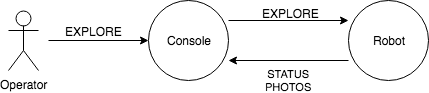
\includegraphics[width=\linewidth]{img/sprint0/system_external_view.png}
\caption{Il sistema osservato da un punto di vista esterno.}
\label{fig:system_external_view}
\end{figure}

Analizzando più nel dettaglio il problema sono emerse le seguenti problematiche: 
\begin{enumerate}
    \item \textbf{Come riceve i comandi la console?}\\
    In questo sistema, l'interazione tra l'operatore e la console può essere modellata a procedure call: l'operatore preme un pulsante su un'interfaccia grafica, la console elabora il comando verificando che esso sia valido e infine chiama la procedura adatta alla sua gestione. 
    Essendo tutto gestito internamente al componente console, risulta inutile utilizzare i paradigmi più complessi (ad esempio, message-based e event-based).
        
    \item \textbf{Come interagiscono console e robot?}\\
    Essendo un sistema distribuito la console e il robot interagiscono attraverso lo scambio di messaggi. I messaggi scambiati tra le due entità sono formalizzati di seguito.
    
       \begin{lstlisting}
//Message from console to robot
Dispatch explore: explore(X)
Dispatch stopExplore: stopExplore(X)
Dispatch backHome: backHome(X)
Dispatch continueExplore: continueExplore(X)
Dispatch backHomeSinceBomb: backHomeSinceBomb(X)
Dispatch continueExploreAfterPhoto: continueExploreAfterPhoto(X)

//Message from robot to console
Dispatch sendPhoto: sendPhoto(X)

//Message from robot to robot
Dispatch reachBag: reachBag(X)

    \end{lstlisting}
   
   \item \textbf{Quali informazioni bisogna mantenere sul modello del robot?}\\
   Il modello del robot può essere descritto attraverso un insieme di informazioni riguardanti:
   \begin{enumerate}
       \item lo stato (per sapere se il robot è fermo, sta andando avanti o indietro, si sta ruotando a destra o sinistra);
       \item la direzione (per sapere sapere come è orientato il robot all'interno della stanza: nord, sud, ovest, est);
       \item la posizione (per sapere dove si trova il robot all'interno della stanza).
   \end{enumerate} 
   
  In particolare, per rintracciare la posizione del robot all'interno della stanza, si utilizza il concetto di griglia, assumendo che esso si muova di passi unitari su di questa.
    
    \item \textbf{Come fa la console ad avere le informazioni riguardanti lo stato del robot?}\\
    Ogni volta che il robot cambia stato emette un evento con le informazioni aggiornate riguardanti il nuovo stato assunto. Tali informazioni verranno poi inviate alla console. L'evento emesso è formalizzato di seguito. 
    
    \begin{lstlisting}
Event modelContent: content(X)

\end{lstlisting}


Lo stato del robot è inizialmente modellato utilizzando Prolog come:

\begin{lstlisting}
//robot state formalisation
state(position(X,Y), direction(D), action(A))

position(X, Y)

direction(west)
direction(east)
direction(north)
direction(south)

action(moving)
action(stop)
action(take_picture)
action(send_photo)

\end{lstlisting}
        
    \item \textbf{Come viene percepito il cambiamento di temperatura della stanza?}\\
    Di default si assume che la temperatura della stanza sia inferiore ad una certa soglia finché al robot non arriva il messaggio di "temperatureTooHigh", il quale indica che la soglia è stata superata. I messaggi inviati al robot sono i seguenti:
   
    \begin{lstlisting}
Dispatch temperatureTooHigh: temperatureTooHigh
Dispatch temperatureOk: temperatureOk

\end{lstlisting}
        
    \item \textbf{Chi invia il messaggio della cambiamento della temperatura?}\\
    Ogni volta che la temperatura supera una certa soglia si scatena un evento che è percepito e gestito dalla console, la quale provvederà all'invio del messaggio "temperatureTooHigh" al robot.
        
    \item \textbf{Come fa il robot ad esplorare la stanza?}\\
     La stanza viene esplorata in maniera autonoma dal robot, quest'ultimo costruisce progressivamente una mappa della stanza riportando su di essa ostacoli fissi, ossia le valigie e i muri, con le relative posizioni e dimensioni. Questo compito può essere suddiviso in due fasi:  
    \begin{itemize}
        \item esplorazione della stanza vuota.
        \item esplorazione con ostacoli fissi.
    \end{itemize}{}
    
    \item \textbf{Quale strategia si può adottare per svolgere l'esplorazione della stanza vuota?}
    È possibile esplorare la stanza vuota in maniera incrementale: il robot coprirà dapprima una piccola area (a lui circostante) che mano a mano si espanderà fino a ricoprire l'intera stanza.
    
    \item \textbf{Quale strategia si può adottare per svolgere l'esplorazione della stanza con ostacoli fissi?}
    È possibile esplorare la stanza con ostacoli fissi in maniera simile a quanto accadrebbe nel caso in cui la stanza fosse vuota: il robot, partendo dalla sua posizione iniziale, esplorerà dapprima la parte di stanza più vicina a lui per poi successivamente espandersi sempre di più. Ogni qual volta il robot si trovi in presenza di un ostacolo, si ricalcolerà un percorso per raggiungere la posizione desiderata sulla griglia. Inoltre, verranno memorizzate le informazioni relative all'ostacolo.
    
    \item \textbf{Come fa il robot a riconoscere un ostacolo?}\\
    Assumiamo che il robot sia dotato nella parte frontale di un sonar e che ogni volta che il sonar rilevi un valore inferiore ad una certa soglia il robot si fermi in quanto si è in presenza di un ostacolo. 
    
    \item \textbf{Da quale prospettiva il robot scatta la foto all'ostacolo?}\\
    Il robot scatta la foto alla valigia esattamente dall'angolazione in cui esso si trova rispetto all'ostacolo nel momento in cui giunge in sua prossimità. Infatti, l'angolazione della foto risulta ininfluente ai fini della valutazione della presenza o meno della bomba, poiché si suppone che il tool utilizzato dalla console esamini il bagaglio con una tecnologia a infrarossi.
    
    \item \textbf{Come fa il robot a tornare nella posizione iniziale?}\\
    La prima cella , ossia (0,0), che il robot memorizza sulla mappa è la sua posizione iniziale, quindi basterà che esso percorra un qualunque tragitto dalla sua posizione attuale alla prima cella memorizzata della mappa per far sì che torni nella sua posizione iniziale.
    
    \item \textbf{In caso di valigia sospetta, cosa fa il robot?}\\
    La valigia sospetta sarà l'ultimo ostacolo memorizzato nella mappa, in quanto quando questo viene rilevato la fase di esplorazione si sospende. 
    Una volta individuata la valigia sospetta, il robot rientrà autonomamente alla base (R-backHomeSinceBomb) al robot. Quando quest'ultimo è tornato alla base (R-waitForHome), esso ripartirà per raggiungere la valigia sospetta, ossia l'ultima memorizzata sulla mappa (R-ReachBag), la inserirà poi in un contenitore e la trasporterà nella sua posizione iniziale (R-bagAtHome). 
    
    \item \textbf{Come fa la console ad interagire con il robot durante la fase di esplorazione?}\\
    Il robot dovrà avere una natura proattiva per gestire autonomamente l'esplorazione della hall e un natura reattiva per ricevere e rispondere prontamente ai messaggi della console.
    
\end{enumerate}

In base all'analisi del problema, si è derivata l'architettura logica di figura \ref{fig:arch_logica}. Al di sopra della linea sono rappresentate le entità principali che compongono il sistema e come queste interagiscono tra di loro , invece, al di sotto delle linea si trovano le relative implementazioni di tali entità.

\begin{figure}  [H]
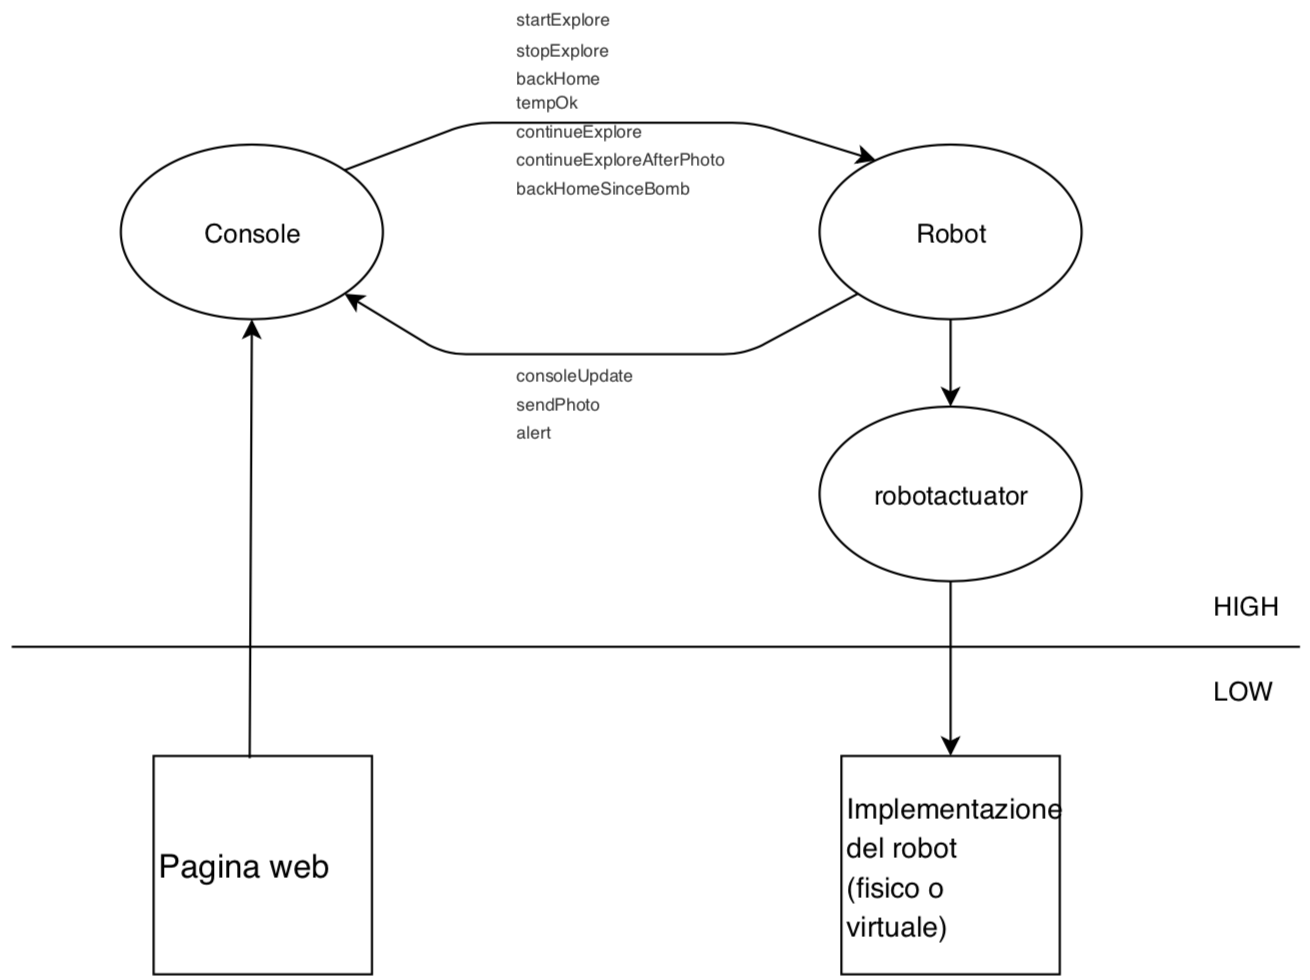
\includegraphics[width=\linewidth]{img/sprint0/arch_logica.png}
\caption{L'architettura logica del sistema.}
\label{fig:arch_logica}
\end{figure}


\subsection{Test Plan}
Nel Test Plan bisogna verificare che:
\begin{itemize}

    \item quando l'utente spinge il pulsante di startExploration e la temperatura della stanza è inferiore ad una soglia fissata, il robot inizi l'esplorazione.
    
     \item quando la console percepisce l'evento del cambio di temperatura, verifica se è ancora adeguata e se è troppo alta invia al robot il messaggio di stopExplore
    
    \item quando il robot riceve il messaggio di explore inizia ad esplorare tutta la stanza;
    
    \item quando il robot riceve il messaggio di stopExplore si ferma nel punto in cui si trova;
     
    \item quando il robot riceve il messaggio di backHome torna nella sua posizione iniziale;
    
    \item quando il robot incontra una valigia non ancora analizzata si ferma, gli scatta una foto e la spedisce con un messaggio alla console (sendPhoto). 
    
    \item quando il robot riceve il messaggio di continueExplore riprende l'esplorazione.
    
    \item quando il robot riceve il messaggio di comeBackSinceBomb torna alla base e passa alla fase di recupero della valigia pericolosa.
    
 
\end{itemize}







    
\begin{lstlisting}
System ddrSys

//robot state update event
Event consoleUpdate: consoleUpdate(X)

//temperature change event
Event tempOk: tempOk(X)

//Message from console to robot
Dispatch explore: explore(X)
Dispatch stopExplore: stopExplore(X)
Dispatch backHome: backHome(X)
Dispatch continueExplore: continueExplore(X)
Dispatch backHomeSinceBomb: backHomeSinceBomb(X)
Dispatch continueExploreAfterPhoto: continueExploreAfterPhoto(X)

//Message from robot to console
Dispatch sendPhoto: sendPhoto(X)

//Message from robot to robot
Dispatch reachBag: reachBag(X)


Context ctx ip [host="localhost" port=8078] -g cyan

QActor console context ctx { 
	
	Plan init normal [
		println("Console intialized")
	]
}

QActor robot context ctx { 
	Plan init normal [
		
		println("Robot intialized")
	]
} 
\end{lstlisting}



\newpage
\subsubsection{Work Plan}
Per la realizzazione dell'intero sistema si procederà in maniera incrementale, raggiungendo ad ogni sprint un determinato obiettivo. Gli obiettivi individuati sono i seguenti:
\begin{enumerate}

    \item creazione di un sistema con un robot in grado di eseguire dei comandi di spostamento (movingForward, movingBackward, rotateLeft, rotateRight, stopped).
        
    \item creazione di un sistema in cui il robot riesca a scambiare messaggi con una web page;

    \item creazione di un sistema con un robot in grado di raggiungere un punto specifico riportato sulla mappa.
    
    \item creazione di un sistema con un robot in grado di esplorare una stanza vuota per poi crearne una mappa. L'esplorazione prevede l'utilizzo di una strategia;
    
    \item creazione di un sistema con un robot in grado di esplorare una stanza contenente ostacoli fissi per poi crearne una mappa;


    
\end{enumerate}

Tale sprint ed i seuguenti sono suddivisi nelle fasi di analisi dei requisiti e analisi del problema, creazione del test plan, modellazione ed implementazione del sistema.


\newpage
\section{Sprint 1}
Il progetto di riferimento per questo sprint è it.unibo.ddrSystem1.

\textbf {OBIETTIVO}: creazione di un sistema con un robot in grado di rispondere a dei comandi. Il robot partendo da una posizione iniziale, dovrà muoversi avanti e indietro, ruotare a destra e sinistra e fermarsi. Inoltre,  il robot dovrà rilevare la presenza delle pareti (ostacoli fissi).

\subsection{Work Plan}
\begin{enumerate}

    \item progettazione del test plan per verificare che il robot si muova correttamente in presenza o meno di ostacoli (muro). 

    \item definizione dei messaggi e degli eventi gestiti dal sistema: messaggi per dare i comandi di movimento e l'evento del sonar del robot; 
    
    \item definizione dell'interazione tra il QActor console e il QActor robot;
    
    \item definizione del comportamento del robot quando percepisce un evento SonarRobot.
    
\end{enumerate}


\subsection{Analisi dei requisiti}
Per la creazione di questo sistema si utilizza un robot dotato di un sonar per rilevare eventuali ostacoli di fronte ad esso. Il robot si muove su una griglia e gli spostamenti del robot sono modellati con un passi unitari, in quanto, ad ogni passo, esso si muove esattamente di una cella. Le dimensioni della cella equivalgono a quelle del robot. 

\subsection{Test plan}
I test da fare sul sistema sono:\\
\newline

\begin{center}

\noindent
\begin{tabular}{|@{}p{10cm}|p{4cm}|}
\hline\\
  &   \\
%\begin{lstlisting}[language=c++,numbers=none]
\begin{lstlisting}[backgroundcolor=\color{white} ]

@Test
	fun initialStateTest(){
		println("%%% initialStateTest %%%")
		solveCheckGoal( robot!!, "model( actuator, robot, state(stopped), direction(south), position(0,0))")
		printRobotState()
		
	}
\end{lstlisting} & Verificare che il robot, prima dell'inizio dell'esplorazione, sia fermo, orientato verso sud e che si trovi nella posizione iniziale (0,0). \\

\hline

\begin{lstlisting}[backgroundcolor=\color{white} ]
@Test
	fun moveTest() {
		println("%%% moveTest  %%%")
		
		rotateRight()
		delay(700)
		
		rotateLeft()
		delay(500)
		
		moveForward()
		delay(700)
		
		moveBackward()
		delay(700)
		
		stoprobot()
		
		solveCheckGoal( robot!!, "model( actuator, robot, state(stopped), direction(south), position(0,0))")
		printRobotState()
 	}
	
\end{lstlisting} & \vspace{0.5ex} Test per verificare che i comandi per spostare il robot vengano eseguiti in maniera corretta. \\

\hline

\begin{lstlisting}[backgroundcolor=\color{white}]


	@Test
	fun wallDetectingTest() {
		moveForward()	//no obstacle assumed
		moveForwardWithWall()
		
		solveCheckGoal( robot!!, "model( actuator, robot, state(stopped), _, _)" )
		printRobotState()
	}


\end{lstlisting} &  \vspace{0.5ex} Verificare che il robot, una volta riconosciuta la presenza di una parete, vada indietro e poi si fermi.\\

\hline
\end{tabular}
\end{center}

\subsection{Model}

Per la realizzazione di questo sprint si è preso come punto di partenza il sistema modellato nello sprint 0, in cui è stato definito più nel dettaglio il comportamento del robot. In particolare si è modellato un robot in grado di ricevere ed eseguire determinati comandi. In questo prototipo le azioni vengono eseguite su una base di conoscenza prolog in modo da tener sempre aggiornato il modello. Il modello è rappresentato come un fatto prolog il quale viene aggiornato ad ogni azione invocata dal sistema. Le azioni sono modellate come predicati prolog.
\\Il modello è: \lstinline {model( actuator, robot, state(S), direction(D), position(X,Y)).} In cui 
\begin{itemize}
    \item S, è la variabile che rappresenta lo stato del sistema e può assumere i seguenti valori: stopped, movingForward, movingBackward, rotateLeft, rotateRight.
    \item D, è la direzione del sistema e può assumere i seguenti valori: north, east, south, ovest.
    \item X,Y sono le coordinate che rappresentano la cella in cui si trova il sistema e possono essere qualsiasi combinazioni di interi compresi tra 0 e il numero massimo di celle della stanza.
\end{itemize}

Le azioni sono :\lstinline {action(robot, move(M)) :- changeModel( actuator, robot, movingForward ).} In cui M è una variabile che può assumere valori diversi a seconda dell'azione che si vuol far eseguire al sistema, può assumere i seguenti valori:
\begin{itemize}
    \item w: se si vuole che il robot si muova in avanti
    \item s: se si vuole che il robot si muova indietro
    \item d: se si vuole che il robot si giri a destra
    \item a: se si vuole che il robot si muova a sinistra
    \item h: se si vuole che il robot si fermi
\end{itemize}

\noindent


    
\begin{tabular}{|@{}p{10cm}|p{5cm}|}
\hline\\
  &   \\
\begin{lstlisting}[backgroundcolor=\color{white}]
Event  sonarRobot: sonarRobot(DISTANCE)	    //from  sonar on robot      
Dispatch: userCmd( CMD ) //Message from console to robot
Dispatch robotCmd: robotCmd (CMD) //Selfsending robot message
\end{lstlisting} &  \vspace{0.5ex} A fianco sono riportati i messaggi e l'evento  che sono stati utilizzati all'interno del sistema. 
\begin{itemize}
\item sonarRobot: evento che si scatena quando il robot si trova in prossimità di una parete 
\item userCmd: messaggio che viene inviato dalla console al robot per far sì che esso cambi il suo stato 
\item robotCmd: messaggio che il robot manda a se stesso nel caso debba effettuare degli spostamenti per evitare un ostacolo.
\end{itemize}{}\\
\hline 
\end{tabular}

\begin{tabular}{|@{}p{10cm}|p{5cm}|}
\hline\\
  &   \\
\begin{lstlisting}[backgroundcolor=\color{white}]
QActor robot context ctx { 
["var obstacle = false"]
	State s0 initial {
		solve (consult ("ddrsys.pl")) 
		solve (consult ("resourceModel.pl")) 
		println("Robot intialized")
		
	} 
	Goto waitForEvents
	  
	State waitForEvents {		} 
	
	Transition t0   whenMsg userCmd  -> handleCmd
					whenMsg robotCmd -> handleCmd
					whenEvent sonarRobot -> handleSonarRobot
 	 
	State handleCmd{  
		printCurrentMessage
		onMsg (userCmd   : userCmd( CMD )){
			solve( action( robot, move($payloadArg(0)) ) ) //change the robot state model
		}
		onMsg (robotCmd   : robotCmd( CMD )){
			solve( action( robot, move($payloadArg(0)) ) ) //change the robot state model
		}
	}
	
	Goto waitForEvents
	
	State handleSonarRobot{
 		printCurrentMessage
 		onMsg ( sonarRobot : sonarRobot(DISTANCE) ){
			["obstacle = Integer.parseInt( payloadArg(0) ) < 10 "]
 		} 	 
 	}
 	
	Goto handeObstacle  if "obstacle" else waitForEvents 
	
	State handeObstacle{		
		println("handleObstacle: going backward")  
 		forward robot -m robotCmd : robotCmd( s ) 		
 			//UPDATE the model : supported action
 			//run itunibo.robot.resourceModelSupport.updateModel( myself, "s" )
 		delay 300
 		println("handeObstacle: stopping")  
	    forward robot -m robotCmd : robotCmd( h )
 			//UPDATE the model : supported action
 			//run itunibo.robot.resourceModelSupport.updateModel( myself, "h" )
  	}
  	
	Goto waitForEvents

} 

\end{lstlisting} &  \vspace{0.5ex} Il robot è formato da tre stati principali:
\begin{itemize}
    \item waitForEvents: nel quale rimane in attesa: di un comando inviato dall'utente (userCmd), di un comando inviato da se stesso (robotCmd), di un evento scatenato dal proprio sonar (sonarRobot) quando si trova in prossimità di un ostacolo.
    \item handleCmd: nel quale il robot gestisce le due tipologie di comandi, in questo caso esegue la stessa azione, ovvero cambia solamente la base di conoscenza del sistema
    \item handeObstacle: nel quale è definita la logica di comportamento a seguito della rilevazione di un ostacolo: si fa andare un po' indietro il robot e poi lo ferma.
\end{itemize}\\

\hline

\end{tabular}





\newpage
\newpage

\section{Sprint 2} 

Il progetto di riferimento per questo sprint è it.unibo.ddrSystem2.

\textbf{OBIETTIVO}: creazione di un robot in grado di esplorare una stanza rettangolare vuota. Il robot, durante l'esplorazione della stanza, dovrà essere in grado di costruire incrementalmente una mappa della stanza.

\subsection{Work Plan}

\begin{enumerate}
    \item utilizzare il simulatore di Soffritti (robot virtuale) per verificare che il sistema creato funzioni correttamente. Nell'effettuare il collegamento tra i due si rimarrà technology independent (robotSupport);
    
    \item utilizzare un robot fisico (realnano) per verificare che il sistema creato funzioni correttamente e che la scelta tecnologica non impatti sull'architettura logica del sistema. Il robot deve essere in grado di muoversi in avanti, in indietro, ruotare a destra, a sinistra e fermarsi, proprio come quello simulato;
    
    \item definizione della strategia di esplorazione della stanza.
    
    \item progettazione del test plan per verificare che il robot riesca a costruire correttamente la mappa della stanza seguendo la strategia scelta.
       
    \item progettazione di una strategia per la creazione della mappa relativa alla stanza. Valutare le diverse possibilità: utilizzo di una base di conoscenza prolog, creazione di una libreria per la gestione della mappa, utilizzo di plannerUtils già fornite. 
 
\end{enumerate}{}


\subsection{Analisi dei requisiti}

\textbf{Cosa si intende per esplorazione della stanza?}\\
Per esplorazione si intende muovere il robot in maniera organizzata e autonoma dentro ad una stanza finché non sono state esplorate tutte le celle. Ad esempio, un risultato che si potrebbe ottenere a fine esplorazione è il seguente:\newline   
r, 1, X,\\
1, 1, X,\\
X, X, X\\

\textbf{Quali informazioni raccoglierà in fase di esplorazione?}\\
Il robot raccoglie le informazioni riguardanti la stanza, in particolare, quali celle sono state visitate, quali ancora no e dove si trovano i muri.

\textbf{Quando il robot inizia ad esplorare autonomamente la stanza?}\\
Quando riceve il comando di "start" (R-startExplore) dalla console.

\textbf{Quando il robot smette di esplorare autonomamente la stanza?}\\
Quando riceve il comando di "stop" (R-stopExplore) dalla console.


\subsection{Analisi del problema}


Esistono varie strategie per permettere al robot di raggiungere l'obiettivo, ognuna di queste prevede che la posizione iniziale (base) del robot coincida con uno degli angoli della stanza e che la distanza percorsa dal robot ad ogni spostamento sia unitaria (in questo caso, l'unità di riferimento è la dimensione del robot). Le strategie vagliate sono le seguenti:
\begin{itemize}
    \item \textbf{a chiocciola}: utilizzando questa strategia il robot esplora in maniera incrementale tutta la superficie della stanza, inizialmente il robot percorre la parte di stanza a lui strettamente adiacente per poi, a mano a mano, espandersi sino ad esplorarla per intero.
    
    \item \textbf{a colonne/righe}: utilizzando questa strategia il robot esplora la stanza muovendosi inizialmente lungo un lato finché non incontra il muro opposto. Una volta incontrato si gira di $90^\circ$ nella direzione in cui non sono presenti muri. Poi si sposta di una unità, si rigira di  $90^\circ$ e procede dritto fino a che non rincontra un altro muro. 
    Al termine dell'esecuzione il robot si deve trovare o nell'angolo opposto (nel caso in cui il numero di colonne/righe fosse dispari) oppure nell'angolo adiacente (nel caso in cui il numero di colonne/righe fosse pari).
    Il modo per implementare questa strategia potrebbe essere quello di creare un robot che percorra tutta la lunghezza di un solo lato della stanza.
    
    \item \textbf{a spirale}: utilizzando questa strategia il robot si muove dapprima lungo le quattro pareti (in maniera oraria e sempre lungo la parente adiacente successiva rispetto a quella che è appena stata esaminata), dopodiché effettua il medesimo tragitto ma restringendo il campo da esplorare. L'esplorazione procede per rettangoli concentrici via via sempre più piccoli e termina quando il robot si trova nel centro della stanza.
\end{itemize}

Esistendo diverse strategie per realizzare questo compito si può pensare di incapsulare la logica di comportamento in più componenti esterni per poi utilizzare quello desiderato.


\subsection{Model}
Si è scelta la strategia della chiocciola per l'esplorazione autonoma in quanto si ritiene che essa sia quella che ottimizza il ritrovamento della bomba, poiché permette di effettuare una ricerca più omogenea e quindi di ritrovare la bomba as soon as possible.
Dato che si ritiene importante dividere la logica di esplorazione del robot dall'attuazione di essa, partendo dal QActor \texttt{robot} modellato nello sprint precedente, si è deciso di suddividerlo in due QActor differenti, ossia:
\begin{itemize}
    \item \texttt{robotmind}: ha il compito di pianificare le azioni necessarie per raggiungere una determinata posizione sulla mappa (vedi funzione \texttt{setGoal(X,Y)}); posizione che diventerà incrementalmente sempre più lontana dalla quella iniziale in quanto si è scelto di esplorare la stanza con la strategia della chiocciola e la cui massima distanza dalla base coinciderà con l'angolo opposto della stanza. Una volta pianificate le azioni per raggiungere un punto della stanza, queste verranno eseguite una alla volta e, in presenza di un ostacolo (muro), una delle azioni fallirà e comporterà il ricalcolo del tragitto che il robot dovrà percorrere (\texttt{vedi State setGoalAfterWall}). 
    
    Il codice di robotmind è riportato nel Listing \ref{lst:robotmind_ddr_sys_2}.
    \item \texttt{robotactuator}: ha il compito di eseguire una alla volta le azioni (vedi \texttt{move(msg(M))} pianificate da \texttt{robotmind}. 
    
    Il codice di robotactuator è riportato nel Listing \ref{lst:robotactuator_ddr_sys_2}.

\end{itemize}
Analizzando i movimenti del robot si è evidenziato che il robot può incontrare un muro solamente quando si muove in avanti, dunque si è introdotto un terzo QActor: \texttt{onestepahead}. In particolare, questo attore riceverà un messaggio \texttt{onestep} (vedi funzione \texttt{attemptToMoveAhead()}) che farà muovere il robot in avanti e controllerà se effettivamente il movimento è possibile. Se il movimento è possibile, in quanto non vi sono ostacoli, ciò verrà notificato a \texttt{robotmind} con un messaggio di \texttt{stepOk} altrimenti \texttt{robotmind} riceverà un messaggio di \texttt{stepFail}.
Il codice di onestepahead è riportato nel Listing \ref{lst:onestepahead_ddr_sys_2}.

L'architettura del sistema è riportata in \cref{fig:sprint2_logic}

\begin{figure} [H]
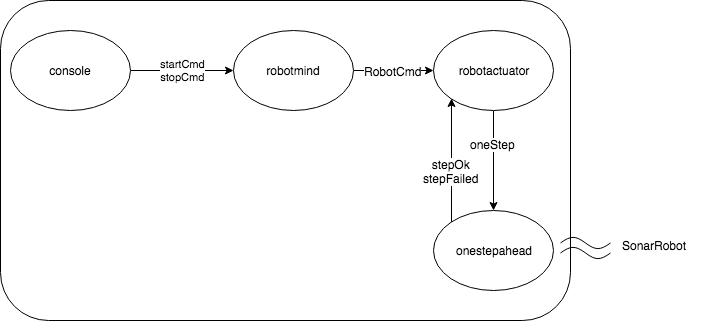
\includegraphics[width=\linewidth]{img/sprint2/sprint2_logic.png}
\caption{Architettura logica del sistema dello sprint 2.}
\label{fig:sprint2_logic}
\end{figure}



\begin{lstlisting}[backgroundcolor=\color{white}, label={lst:robotmind_ddr_sys_2}, caption={Codice di QActor robotmind in ddrSystem2} ]

QActor robotmind context ctx { 
["var Curmove     = \"\"  
var IterCounter = 0 
var backHome = false
var maxX = 0
var maxY = 0
var finish = false

//VIRTUAL ROBOT
var StepTime   = 330	 
 
var Tback       = 0
"]
	State s0 initial {
		println("&&&  robotmind STARTED")
		solve (consult ("ddrsys.pl")) 
		solve (consult ("resourceModel.pl")) 
		println("Robot intialized")
		run itunibo.planner.plannerUtil.initAI()
		println("INITIAL MAP") 
		run itunibo.planner.plannerUtil.showMap() 
		
	} 
	
	Goto waitForStart
	
	State waitForStart {	printCurrentMessage }
	
	Transition t0  whenMsg startCmd  -> startExploration
				   whenMsg startTest -> startExplorationTest
	
	State startExplorationTest {
		["finish = true
		  backHome = false

		  var x = \"\"
		  var y = \"\"	"]
		println("&&&  exploration TEST")
		
		printCurrentMessage		        
 		onMsg( startTest : startTest(X, Y) ) { 
 			[" x =payloadArg(0) 
			   y =payloadArg(1) "]
		run itunibo.planner.plannerUtil.setGoal(x,y)
		run itunibo.planner.moveUtils.doPlan( myself ) //moves stored in actor kb	
 		}
	}
	Goto doPlan
	
	
	State startExploration {
		println("&&&  exploration STARTED")
		run itunibo.planner.plannerUtil.setGoal("1","1")
		run itunibo.planner.moveUtils.doPlan( myself ) //moves stored in actor kb
	}
	
	Goto doPlan
	
	//raggiungo la cella
	State doPlan {	
		run itunibo.planner.plannerUtil.showMap() 
		solve( retract( move(M) ) ) 	//consume a move
		ifSolved {  ["Curmove = getCurSol(\"M\").toString()"]  }
		 else { ["Curmove=\"nomove\" "]  }
	}  
	
	Goto handlemove if "(Curmove != \"nomove\")" else choose
	
	State handlemove {}
	
	Goto domove if "(Curmove != \"w\")" else attempttogoahead
	
	State domove {
		run itunibo.planner.moveUtils.doPlannedMove(myself, Curmove)
		forward robotactuator -m robotCmd : robotCmd(\$Curmove)
		delay 700
		forward robotactuator -m robotCmd : robotCmd(h)
	}
	
	Goto doPlan
	
	//roomboundaryplanning.qak
	State attempttogoahead {	
		run itunibo.planner.moveUtils.attemptTomoveAhead(myself, StepTime)
	}
	Transition t0   whenMsg stepOk   -> stepDone   
					whenMsg stepFail -> stepFailed 
	 
 	State stepDone{  
 		run itunibo.planner.moveUtils.doPlannedMove(myself, "w")	
 	}
 	
 	Goto doPlan
 	
 	State stepFailed{
 		println("&&&  FOUND WALL")
["var TbackLong = 0L"]		 
 	  	
		//printCurrentMessage		        
 		onMsg( stepFail : stepFail(Obs, Time) ) { 
 			["Tback=payloadArg(1).toLong().toString().toInt() / 2
			TbackLong = Tback.toLong()"]
 			println("stepFailed \${payloadArg(1).toString()}")
 		}
  		
 		println(" backToCompensate stepTime=\$Tback")
 		forward robotactuator -m robotCmd : robotCmd(s)
		delayVar TbackLong
		forward robotactuator -m robotCmd : robotCmd(h)
		delay 700
 //--------------------------------------------------
 		run itunibo.planner.plannerUtil.wallFound()
 	
	}   
	
	//Goto endOfJob //**checkWallTest
	Goto setGoalAfterWall
	
	State setGoalAfterWall{
		solve( retractall( move(_) ))
	["
	if( itunibo.planner.plannerUtil.getDirection() == \"downDir\" ){ 
		maxY = itunibo.planner.plannerUtil.getPosY()
		if(maxX == 0 ){
			itunibo.planner.plannerUtil.setGoal(IterCounter, maxY)
		} else {itunibo.planner.plannerUtil.setGoal(maxX, maxY)}
	} 
	else if( itunibo.planner.plannerUtil.getDirection() == \"rightDir\" ){ 
		maxX = itunibo.planner.plannerUtil.getPosX()
		if (maxY == 0 ){
			itunibo.planner.plannerUtil.setGoal(maxX, IterCounter)
		} else { itunibo.planner.plannerUtil.setGoal(maxX, maxY) }
	} else {
		itunibo.planner.plannerUtil.setGoal(0, 0)
	}
	"]
		run itunibo.planner.moveUtils.doPlan( myself )
	}
	
	Goto doPlan

	
	State choose {}
	Goto goBackHome if "backHome" else nextStep
	
 	//torno a casa
	State goBackHome{
	["backHome = false"]
		println("&&&  returnToHome")
 		//solve( retractall( move(_) ))		//clean the actor kb
 		run itunibo.planner.plannerUtil.setGoal(0,0)
  		run itunibo.planner.moveUtils.doPlan( myself )
	
  		delay 700
    }  
	
	Goto doPlan
	 
	State nextStep {}

	Goto endOfJob if "finish" else calculatenextstep
	
	State calculatenextstep{
["IterCounter++
	backHome = true
	if (maxX == 0 && maxY == 0){ itunibo.planner.plannerUtil.setGoal(IterCounter,IterCounter) }
	else if( maxX != 0 && maxY == 0 ){ itunibo.planner.plannerUtil.setGoal(maxX,IterCounter) } 
	else if( maxX == 0 && maxY != 0 ){ itunibo.planner.plannerUtil.setGoal(IterCounter, maxY) } 
	else {
 		itunibo.planner.plannerUtil.setGoal(maxX, maxY)
		finish = true 
}
"]
		println("&&&  nextStep")
 		run itunibo.planner.moveUtils.doPlan( myself )
	}
	Goto doPlan
	
	State endOfJob{
		["if (maxX != 0 && maxY != 0) {itunibo.planner.plannerUtil.fixwalls(maxX, maxY)}"]
		
		println("FINAL MAP")   
 		run itunibo.planner.plannerUtil.showMap() 
		println("&&&  planex0 ENDS")
 	}

}

\end{lstlisting}

\begin{lstlisting}[backgroundcolor=\color{white}, label={lst:robotactuator_ddr_sys_2}, caption={Codice di QActor robotactuator in ddrSystem2} ]


QActor robotactuator context ctx {	 
	State s0 initial {  
		["  
//CREATE A PIPE for the sonar-data stream
val filter = itunibo.robot.sonaractorfilter( \"sonaractorfilter\" , myself  ) 
val logger = itunibo.robot.Logger(\"logFiltered\")
filter.subscribe(logger)  

"] 	 	
 			  
   		solve( consult("basicRobotConfig.pl") )   
 		solve( robot(R, PORT) )  //R = virtual | realmbot | realnano
  		ifSolved { 
     		println( "USING ROBOT : \${getCurSol(\"R\")},  port= \${getCurSol(\"PORT\")} " )
  			run itunibo.robot.robotSupport.create( myself, @R, @PORT, filter )
  		} 
  		else{ println("no robot") }
    		
   		run itunibo.robot.robotSupport.move( "msg(a)" )
   		delay 700
   		run itunibo.robot.robotSupport.move( "msg(d)" )
   		delay 700
   		run itunibo.robot.robotSupport.move( "msg(h)" )
 	}  
	Goto waitCmd   
 	 
	State waitCmd{  } //robotCmd comes from a console OUTSIDE this (sub)system
	Transition t0  whenMsg   robotCmd  -> handleRobotCmd
	
	State handleRobotCmd{ //does not handle alarms 
		printCurrentMessage 
		onMsg( robotCmd : robotCmd( MOVE ) ) { //MOVE = w | a | s | d | h
			run itunibo.robot.robotSupport.move( "msg(\${payloadArg(0)})" ) 
		}	
 	}   
	Goto waitCmd 
}  

\end{lstlisting}

\begin{lstlisting}[backgroundcolor=\color{white}, label={lst:onestepahead_ddr_sys_2}, caption={Codice di QActor onestepahead in ddrSystem2} ]

QActor onestepahead context  ctx {
[" 
var foundObstacle = false; 
var StepTime = 0L; 
var Duration=0 
"]  
	State s0 initial {	   
		["foundObstacle = false "]
	} 
	Transition t0 whenMsg onestep -> doMoveForward
 
	State doMoveForward{		 
		onMsg( onestep : onestep( TIME ) ) {
			["StepTime = payloadArg(0).toLong()"]    		
			forward robotactuator -m robotCmd : robotCmd(w)
	 		["startTimer()"] //startTimer is built-in in the actor
	 		
		}      
	}          
	Transition t0 whenTimeVar StepTime  -> endDoMoveForward		
 		           whenEvent sonarRobot -> stepFail  
 		    
	State endDoMoveForward{
		forward robotactuator -m robotCmd : robotCmd(h)
		forward robotmind -m stepOk : stepOk
	}
	Goto s0
	  

	
	State stepFail{ 
		["Duration=getDuration()"]  //getDuration is built-in in the actor
		printCurrentMessage
		println("onestepahead stepFail Duration=$Duration ")
		
		forward robotmind -m stepFail : stepFail(obstacle, $Duration)
	}
	Goto s0  
}    


\end{lstlisting}



\subsection{Test plan}
I test da fare sul sistema sono:
%\newline

\begin{center}
    

\begin{tabular}{|@{}p{10cm}|p{5cm}|}
\hline\\
  &   \\
\begin{lstlisting}[backgroundcolor=\color{white}]
    @Test
	fun cheGoalTest() {
		
		GlobalScope.launch{
 			console!!.forward("startTest", "startTest(1,1)", "robotmind")
 		}
		delay(10000)
		val pos = getRobotPos()
		assertTrue(pos == "(1,1)")
		
		printRobotState()
	}
\end{lstlisting} &  \vspace{0.5ex}  verificare che il robot virtuale riesca a raggiungere un determinato obiettivo (i.e. cell(1,1)) . \\
\hline 

%\end{tabular}

%\begin{tabular}{|@{}p{10cm}|p{5cm}|}
%\hline\\
 % &   \\
\begin{lstlisting}[backgroundcolor=\color{white}]
    @Test
	fun checkWallTest() {
		
		GlobalScope.launch{
 			console!!.forward("startTest", "startTest(0,8)", "robotmind")
 		}
		delay(5000)
		val state = getRobotState()
		assertTrue(state == "downDir, (0,7)")
		printRobotState()
		
	}
\end{lstlisting} &  \vspace{0.5ex}  verificare che il robot virtuale, una volta riconosciuta la presenza di una parete, si riposizioni nella cella immediatamente precedente e poi si fermi. \\
\hline 

\begin{lstlisting}[backgroundcolor=\color{white}]
	@Test
	fun finalMapTest() {
		
		var testRoomMap = """|r, 1, 1, 1, 1, 1, 1, 1, X,  
                        |1, 1, 1, 1, 1, 1, 1, 1, X, 
                        |1, 1, 1, 1, 1, 1, 1, 1, X, 
                        |1, 1, 1, 1, 1, 1, 1, 1, X, 
                        |1, 1, 1, 1, 1, 1, 1, 1, X, 
                        |1, 1, 1, 1, 1, 1, 1, 1, X, 
                        |1, 1, 1, 1, 1, 1, 1, 1, X, 
                        |1, 1, 1, 1, 1, 1, 1, 1, X, 
                        |X, X, X, X, X, X, X, X, X, """
          
		GlobalScope.launch{
 			console!!.forward("startCmd", "startCmd", "robotmind")
 		}
		delay(99000)
		assert(itunibo.planner.plannerUtil.getMap() = = testRoomMap)
	}
\end{lstlisting} &  \vspace{0.5ex}   verificare la correttezza della mappa prodotta dal robot al termine dell'esplorazione: quest'ultima dovrà combaciare con quella effettiva della stanza per quanto riguarda dimensioni e numero di celle. \\
\hline 

\end{tabular}
\end{center}




\newpage
\section{Sprint 3} 

I progetti di riferimento per questo sprint sono:
\begin{itemize}
    \item it.unibo.ddrSystem3 (lo stato del robot è modellato con prolog e visualizzato sulla web page)
    \item it.unibo.ddrSystem4 (lo stato del robot è modellato con prolog e CoAP e visualizzato sulla web page)
    \item it.unibo.frontend (interfaccia web)
\end{itemize}


\textbf{OBIETTIVO}: rendere le informazione del sistema (robot e stanza) accessibili via web utilizzando il protocollo standard RESTful.

\subsection{Work Plan}
\begin{enumerate}
\item rendere le informazioni del sistema accessibili via web;
\item creazione di un'interfaccia node dove:
    \begin{itemize}
        \item inviare comandi al sistema (start, ossia (R-startExplore) e stop, ossia R-stopExplore); 
        \item visualizzare lo stato del sistema (in particolare lo stato del robot e le informazioni da lui raccolte, ossia R-consoleUpdate);
    \end{itemize}
\end{enumerate}

\subsection{Analisi del problema} 
Le informazioni del sistema che devono essere visualizzate sulla web page riguardano il robot e la stanza.
Fino a questo momento lo stato del robot è stato gestito mediante una base di conoscenza prolog (\texttt{resourceModel.pl}). Questa prima scelta è stata effettuata in quanto la risorsa era acceduta solamente dall'interno del sistema (test).
Per quanto riguarda la stanza, essa è stata finora modellata in Java mediante la libreria \texttt{it.unibo.planner}.
Nasce ora l'esigenza di accedere a tali risorse mediante internet rendendo quindi visibile lo stato del robot e quello di avanzamento di esplorazione della stanza sulla pagina web (\texttt{frontend.js}). Di conseguenza viene spontaneo modellare queste risorse utilizzando il protocollo standard RESTful. La tecnologia scelta a tale scopo è CoAP.

\subsection{Model} 
Volendo dare la possibilità di accedere alle informazioni del sistema via web il sistema può essere considerato un sistema IoT. Dunque si ritiene importante  utilizzare un'architettura di tipo esagonale in cui il modello delle risorse è al centro e ogni cambiamento del sistema avviene conseguentemente ad una modifica del modello. 
Si è introdotto dunque un nuovo QActor (resourcemodel) responsabile della gestione del modello delle risorse.
L'interazione tra la web page e il sistema verrà gestita anche utilizzando un approccio di tipo publish/subscribe, in particolare utilizzando MQTT.

\begin{center}
\begin{longtable}{|p{7cm}|p{7cm}|}
\caption{QActor resourcemodel in exploration.qak}
\label{tbl:technical-risks}\\
\hline
\textbf{Codice} & \textbf{Descrizione}  \\ 
\hline
\endfirsthead
\multicolumn{2}{c}
{\tablename\ \thetable\ -- \textit{Continued from previous page}} \\
\hline
\textbf{Codice} & \textbf{Descrizione}  \\ 
\hline
\endhead
\hline \multicolumn{2}{r}{\textit{Continued on next page}} \\
\endfoot
\endlastfoot

\begin{lstlisting}[backgroundcolor=\color{white} ]

Actor resourcemodel context robotResourceCtx{

	State s0 initial {
		solve( consult("sysRules.pl")	 )
		solve( consult("resourceModel.pl")	 )
		solve( showResourceModel )
		run itunibo.coap.modelResourceCoap.create( myself, "resourcemodel" ) //CoAP access
	}
	Goto waitModelChange

	State waitModelChange{ }
	Transition t0 whenMsg modelUpdate -> updateModel //forward from robotmind

	State updateModel{
		printCurrentMessage
		onMsg( modelUpdate : modelUpdate(robot,V ) ) {
		
			run itunibo.robot.resourceModelSupport.updateRobotModel( myself, payloadArg(1) )
			solve( showResourceModel )
		}
		onMsg( modelUpdate : modelUpdate(sonarRobot,V ) ) {
			run itunibo.robot.resourceModelSupport.updateSonarRobotModel( myself, payloadArg(1) )
		}
		onMsg( modelUpdate : modelUpdate(roomMap,V ) ) {  //JULY19
			//println("modelUpdate roomMap")
			run itunibo.robot.resourceModelSupport.updateRoomMapModel( myself, payloadArg(1) )
		}
	}
    Goto  waitModelChange
}



\end{lstlisting}
& 

il QActor resourcemodel inzialmente crea la risorsa CoAP. Il CoAP server, una volta fatto partire, renderà accessibile tale risorsa all'indirizzo   \texttt{coap://localhost:5683/resourcemodel} ed i CoAP client (i.e. la web page) potranno essere notificati quando lo stato della risorsa cambia (\texttt{fun updateState( modelitem : String )} nella classe \texttt{it.unibo.coap.modelResourceCoap.kt})
Ogni qualvolta il QActor resourcemodel riceve da QActor robotmind un messaggio di \texttt{modelUpdate} Il QActor resourcemodel prima emetterà un evento \texttt{modelContent} per notificare la web page (gestito tramite MQTT) ed aggiornarla con le nuove informazioni,  poi procederà con l'aggiornamento della risorsa CoAP. 

Il messaggio di modelUpdate può corrispondere ad uno dei seguenti formati:
\begin{itemize}
    \item  \texttt{modelUpdate : modelUpdate(robot,V )}
    \item  \texttt{modelUpdate : modelUpdate(sonarRobot,V )} 
    \item  \texttt{modelUpdate : modelUpdate(roomMap,V )}
\end{itemize}

\\ \hline

\begin{lstlisting}[backgroundcolor=\color{white} ]


QActor robotmind context robotMindCtx { 

...

State waitForStart {
	}
	
	Transition t0  whenMsg startCmd  -> startExploration 
				 

	State startExploration {
		println("&&&  exploration STARTED")
		run itunibo.planner.plannerUtil.setGoal("1","1")
		run itunibo.planner.moveUtils.doPlan( myself ) //moves stored in actor kb
	}
	
...

\end{lstlisting}
&

Per inviare il comando di "start" si è reso necessario far comunicare la web page con il QActor robotmind. In particolare, quando verrà premuto il bottone "start" sulla web page, il publisher (ossia le web page) pubblicherà il messaggio \texttt{msg(startCmd,dispatch,js,robotmind,
startCmd,1)} sulla topic \texttt{unibo/qak/robotmind} (topic alla quale il QActor robotmind ha fatto la subscribe al momento della sua creazione)) dell'MQTT broker. Dopodiché, il QActor robotmind, ricevuto il messaggio \texttt{startCmd}, darà il via all'esplorazione automatizzata della stanza così come la si era strutturata nello sprint precedente (punto 3 del work plan).



\\\hline

\begin{lstlisting}[backgroundcolor=\color{white} ]


QActor robotmind context robotMindCtx { 

    ...
    
	//raggiungo la cella
	State checkStop {	}
	
	Transition t1 whenTime 100  -> doPlan		
 		           whenMsg stopCmd -> handleStop  
 		            
 	...
 	 
 	State handleStop{
		onMsg(stopCmd : stopCmd) {
			forward robotactuator -m robotCmd : robotCmd(h)
			forward resourcemodel -m modelUpdate : modelUpdate(robot, h)
		}
	}
	
	Transition t3  whenMsg startCmd  -> doPlan
}


\end{lstlisting}
&
Similmente accade per il comando di "stop", in quanto  il publisher (ossia le web page) pubblicherà il messaggio \texttt{msg(stopCmd,dispatch,js,robotmind,
stopCmd,1)} sulla topic \texttt{unibo/qak/robotmind} dell'MQTT broker.
Dopodiché, il QActor robotmind, ricevuto il messaggio \texttt{stopCmd}, arresterà l'esplorazione. Sarà possibile riprendere l'esplorazione premendo sul comando "start".
\\\hline

\begin{lstlisting}[backgroundcolor=\color{white} ]

QActor resourcemodel context robotResourceCtx{
...
State updateModel{
        ...
		onMsg( modelUpdate : modelUpdate(robot,V ) ) {
			run itunibo.robot.resourceModelSupport.updateRobotModel( myself, payloadArg(1) )
			solve( showResourceModel )
		}
        ...
}


\end{lstlisting}
&

Per visualizzare le informazioni relative al robot e alla stanza, si utilizza la topic\texttt{unibo/qak/events} sulla quale il QActor resourcemodel (publish) pubblicherà l'evento \texttt{( "modelContent" , "content(robot(\$RobotState, \$RobotDir, \$RobotPos ))")} ogni qualvolta riceva un messaggio \texttt{forward resourcemodel -m modelUpdate  :  modelUpdate( robot, \$Curmove)} dal QActor robotmind. Dopodichè, la web page (subscribe), verrà notificata del cambiamento delle informazioni e provvederà ad aggiornarle.
 

\\\hline

\begin{lstlisting}[backgroundcolor=\color{white} ]

QActor resourcemodel context robotResourceCtx{
...
State updateModel{
        ...
		onMsg( modelUpdate : modelUpdate(roomMap,V ) )
			run itunibo.robot.resourceModelSupport.updateRoomMapModel( myself, payloadArg(1) )
		}
        ...
}

\end{lstlisting}
&

Il meccanismo attraverso il quale vengono visualizzate le info raccolte dal robot in merito all'esplorazione della stanza rimane invariato rispetto a quello appena descritto per lo stato del robot. Ciò che cambia è la tipologia di evento ed il formato del messaggio infatti il QActor resourcemodel emetterà un evento del tipo \texttt{"modelContent", "content( roomMap( state('\$content')))} dopo aver ricevuto dal QActor robotmind \texttt{forward resourcemodel -m modelUpdate  : modelUpdate( roomMap, \$Map )} 
\\\hline

\end{longtable}
\end{center}


L'architettura del sistema è riportata in \cref{fig:arch_logica_3}.


    

\begin{figure}[H]
  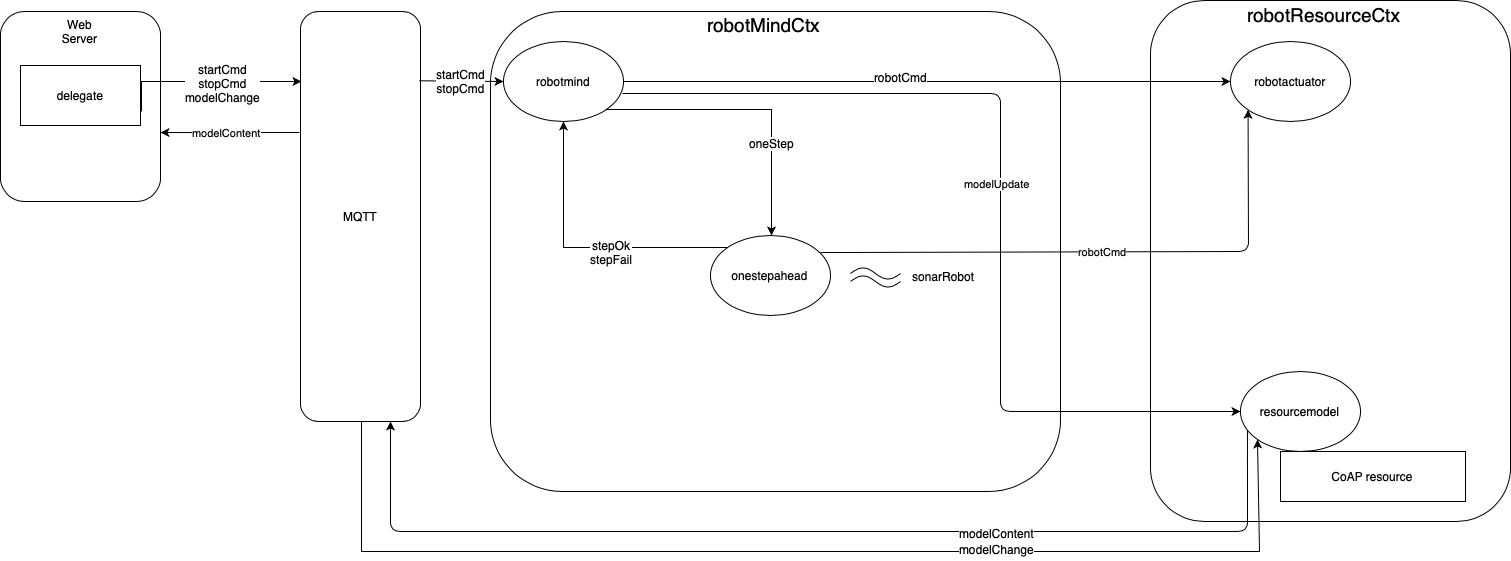
\includegraphics[width=\textwidth]{img/sprint3/arch_logica_3.png}
  \caption{L'architettura del sistema.}
  \label{fig:arch_logica_3}
\end{figure}

\subsection{Test plan}

Verificare il corretto funzionamento del sistema:

\begin{itemize}
\item alla pressione del tasto start/stop sulla web page il sistema parte/si ferma e lo stato della risorsa CoAP cambia coerentemente;
\item le informazioni visualizzate sulla web page corrispondano allo stato reale del sistema;
\end{itemize}{}



\newpage
\section{Sprint 4} 

Il progetto di riferimento per questo sprint è it.unibo.ddrSystem5.

\textbf{OBIETTIVO}: creazione di un sistema con un robot che, data una stanza con ostacoli (sia muri sia valigie), la esplori in maniera autonoma e ne costruisca una mappa. Sulla mappa dovranno essere evidenziati tutti gli ostacoli individuati. 

\subsection{Work Plan}
\begin{enumerate}
\item definizione di valigia come nuova entità del sistema;
\item definizione di "fine esplorazione" di una stanza con ostacoli fissi (muri e valigie);
\item creazione di una strategia per la gestione degli ostacoli;
\item creazione di una strategia per terminare l'esplorazione di una stanza con ostacoli.
\end{enumerate}

\subsection{Analisi dei requisiti}

\textbf{Che cosa si intende per valigia?}\\
La valigia rappresenta un ostacolo fisso disposto all'interno della stanza. Essa può trovarsi in mezzo alla stanza oppure adiacente ad 1 o 2 pareti. Una valigia è un ostacolo che può essere aggirato dal robot, quindi non sarà possibile per il robot esplorare la cella occupata della valigia, ma solo le celle adiacenti.
Nel caso in cui un ostacolo si trovi parzialmente su una cella, essa viene comunque considerata dal robot interamente occupata da un ostacolo.
Inoltre, in questo sistema non si tiene conto della differenza tra un muro ed una fila lunga di valigie: entrambi determinano il confine della stanza. Perciò, in presenza di un ostacolo, se il robot riesce a raggiungere con un altro percorso il proprio obiettivo, allora continuerà l'esplorazione, in caso negativo significherà che il robot ha individuato i confini.


\textbf{Che cosa si intende per "fine esplorazione"?}\\
L'esplorazione si considera terminata dopo che il robot ha individuato i confini della stanza, esplorato tutte le celle segnalate con uno 0 sulla mappa ed è tornato nella sua posizione iniziale (0,0).

\subsection{Analisi del probelma}

La problematica principale che emerge è la
gestione degli ostacoli della stanza. In questo sprint sono state individuate due possibili strategie che prevedono l'utilizzo di un sonar posizionato sulla parte frontale del robot. Tali strategie sono:
\begin{itemize}
    \item il robot, in presenza di un ostacolo prova ad aggirarlo andando alla sua sinistra (questo processo può essere iterato, nel caso in cui un ostacolo occupi più di una cella). Se il robot ci riesce, considera l'ostacolo una valigia, altrimenti un muro. In figura \cref{fig:go_around_obstcl_strategy} sono riportate le varie casistiche in cui il robot si potrebbe trovare.
    \item il robot, in presenza di un ostacolo, calcola un percorso alternativo per raggiungere l'obiettivo. Nel caso in cui non vi siano percorsi disponibili, significa che sono stati individuati i confini della stanza. Altrimenti significa che il robot ha individuato una valigia in mezzo alla stanza o adiacente ad una parete.

\end{itemize}

Analizzate le due possibili soluzioni si è giunti alla conclusione che la logica applicativa della seconda strategia fosse la più semplice tra le due in quanto permette al robot di gestire nella maniera più opportuna gli ostacoli presenti. Inoltre, si è ritenuto che questa strategia rappresenti una soluzione più elegante in quanto permette di non stravolgere il sistema di partenza.

\begin{figure}[H]
  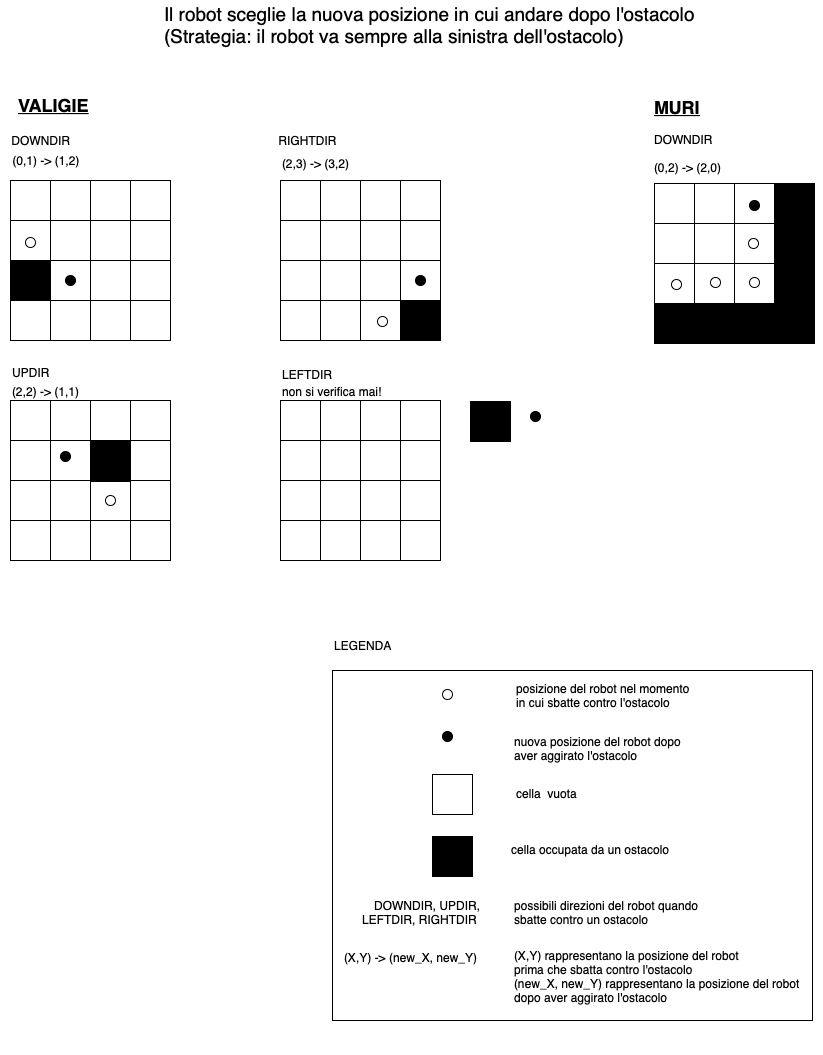
\includegraphics[scale=0.35]{img/sprint4/go_around_obstcl_strategy.png}
  \caption{Le varie casistiche che il robot potrebbe dover affrontare.}
  \label{fig:go_around_obstcl_strategy}
\end{figure}

Un'altra problematica riguarda la gestione della fase di "fine esplorazione" in quanto, una volta che il robot ha individuato i confini della stanza, potrebbero comunque essere rimaste delle celle inesplorate (riportate con uno 0 sulla mappa). Per risolvere questo problema è necessario che il robot le visiti una ad una.

\subsection{Model}

La logica di funzionamento di robotmind dovrà gestire la nuova tipologia di ostacolo (valigia). Partendo dal presupposto che il robot ispezionerà la stanza utilizzando la strategia della chiocciola (già implementata nello Sprint 2), la nuova logica applicativa del robot dovrà eseguire i seguenti passi:
\begin{enumerate}
\item  ogni volta che il robot sbatte contro un ostacolo, quest'ultimo viene segnato sulla mappa con una X (già implementata nello Sprint 2);
\item il robot elabora un nuovo piano per provare a raggiungere il goal prefissato, se il piano fallisce ne calcola uno nuovo;
\item quando il robot esaurisce i piani disponibili  per raggiungere il goal, significa che le coordinate del goal non rientrano nelle dimensioni della stanza e che entrambe i muri (muro lato sud e lato est) della stanza sono stati individuati;
\item in ultimo, il robot finisce di controllare le celle della stanza rimaste inesplorate (rappresentate con uno 0 sulla mappa). Per ogni cella ancora inesplorata, il robot verifica se la cella è vuota oppure occupata da un ostacolo. \end{enumerate}

Inoltre, la logica applicativa che riguarda la realizzazione effettiva del piano (doPlan) ed il suo successo o fallimento è stata estrapolata da robotmind ed incapsulata in un nuovo attore (planexecutor), che dato un goal (es. il robot deve raggiungere la posizione (2,2) nella stanza), verifichi se il goal può essere portato a termine e notifichi l'attore (robotmind) del suo successo o fallimento. Il codice di planexecutor è riportato nel Listing \ref{lst:planexecutor-ddr-sys-5}. Il Listing \ref{lst:robotmind-ddr-sys-5} contiene i messaggi sui quali starà in attesa robotmind a fronte della nuova spartizione dei compiti tra lui stesso e planexecutor.
Per quanto riguarda la gestione degli eventi del sonar si è ritenuto opportuno creare un QActor dedicato, denominato sonahandler. Questo QActor, ogni volta che cattura un evento sonarRobot, non invia alcun messaggio nel caso in cui il valore sia maggiore di una certa soglia, poichè significa che non è presente un ostacolo di fronte al robot, in caso contrario invia un messaggio all'attore onestepahead. 

\begin{lstlisting}[backgroundcolor=\color{white}, label={lst:planexecutor-ddr-sys-5}, caption={"Codice di planexecutor in ddrSystem5"}]

QActor planexecutor context robotMindCtx {
	["
		var Curmove     = \"\"  
		var Map = \"\"
		var Tback = 0
		var StepTime   = 330 
		//var StepTime   = 700 //fisico 

    "]
	State s0 initial {} 

	Transition t0  whenMsg doPlan  -> loadPlan
				 
	State loadPlan {
		printCurrentMessage
 		run itunibo.planner.moveUtils.doPlan( myself ) //moves stored in actor kb
	}
				 	
	Goto doPlan
	
 	State doPlan {	}
 	
	Transition t1 whenTime 50  -> doPlan1 		
 		          whenMsg stopCmd -> stopAppl
 		          
 	State stopAppl {
 		forward robotactuator -m robotCmd : robotCmd(h)
 		forward resourcemodel -m modelUpdate  : modelUpdate( robot, h ) 
 		solve(retractall( move(_)))
 	} 
 	
 	Goto s0
 	
 	State doPlan1{
 	
		["Map =  itunibo.planner.plannerUtil.getMapOneLine()"]
		forward resourcemodel -m modelUpdate  : modelUpdate( roomMap, $Map )
		run itunibo.planner.plannerUtil.showMap() 
		
		solve( retract( move(M) ) ) 	//consume a move
		ifSolved {  ["Curmove = getCurSol(\"M\").toString()"]  }
		else { ["Curmove=\"nomove\" "]  }

	}  
	
	Goto handlemove if "(Curmove != \"nomove\")" else planOk
	
	State planOk {
		forward robotactuator -m robotCmd : robotCmd(h)
		forward resourcemodel -m modelUpdate  : modelUpdate( robot, h ) 
		forward robotmind -m planOk : planOk 
	}
	
	Goto s0
	
	State handlemove {}
	
	Goto domove if "(Curmove != \"w\")" else attempttogoahead
	
	State domove {
		
		run itunibo.planner.moveUtils.doPlannedMove(myself, Curmove)
		forward robotactuator -m robotCmd : robotCmd($Curmove)
		delay 500 //fisico  
		forward robotactuator -m robotCmd : robotCmd(h)
	
		forward resourcemodel -m modelUpdate  : modelUpdate( robot, $Curmove ) 
	}
	
	Goto doPlan
	
	//roomboundaryplanning.qak
	State attempttogoahead {	
		forward resourcemodel -m modelUpdate  : modelUpdate( robot, w ) 
		run itunibo.planner.moveUtils.attemptTomoveAhead(myself, StepTime)
	}
	
	Transition t2   whenMsg stepOk   -> stepDone   
					whenMsg stepFail -> stepFailed
					 
 	State stepDone{  
 		forward resourcemodel -m modelUpdate  : modelUpdate( robot, h ) 
 		run itunibo.planner.moveUtils.doPlannedMove(myself, "w")	
 		
 	}
 	
 	Goto doPlan
 	
 	State stepFailed{
 		println("&&&  OBSTACLE FOUND") 
		["var TbackLong = 0L"]		 
 	  	
		//printCurrentMessage		        
 		onMsg( stepFail : stepFail(Obs, Time) ) { 
 			["Tback= (payloadArg(1).toLong().toString().toInt()*0.85 ).toInt()
			TbackLong = Tback.toLong()"]
 		}
  		
 		println(" backToCompensate stepTime=$Tback")
 		forward resourcemodel -m modelUpdate  : modelUpdate( robot, s ) 
 		forward robotactuator -m robotCmd : robotCmd(s)
		
		delayVar TbackLong
		
		forward robotactuator -m robotCmd : robotCmd(h)
		forward resourcemodel -m modelUpdate  : modelUpdate( robot, h ) 
		
		forward robotmind -m planFail : planFail 
		solve(retractall( move(_)))	
	}
	Goto s0	
}


\end{lstlisting}


\begin{lstlisting}[backgroundcolor=\color{white}, label={lst:robotmind-ddr-sys-5}, caption={"Codice di robotmind in ddrSystem5"}]



QActor robotmind context robotMindCtx { 

    ...

	State startExploration {
		println("&&&  exploration STARTED")
	
		run itunibo.planner.plannerUtil.setGoal(X,Y)
		forward planexecutor -m doPlan : doPlan($X,$Y)
	}
	
	Transition t1 ...
	              whenMsg planOk -> nextGoal
				  whenMsg planFail -> checkIfObstacle
				  
	State nextGoal {
		if "backHome" {
			["
			backHome = false
			X = 0
			Y = 0
			iterCounter++"]
		}
		else {
		["
			backHome = true
			X = iterCounter
			Y = iterCounter
		"]
		}
	}
	
	...
	
	State checkIfObstacle {
		println("---CheckIfObstacle---")
		run itunibo.planner.moveUtils.setObstacleOnCurrentDirection(myself)
		run itunibo.planner.plannerUtil.resetGoal(X,Y)
		run itunibo.planner.moveUtils.setObstacleOnCurrentDirection(myself)
		["plan = itunibo.planner.plannerUtil.doPlan()"]	
		
	}
	
    ...
}

\end{lstlisting}

L'architettura del sistema è riportata in \cref{fig:arch_logica_4}.

\begin{figure}[H]
  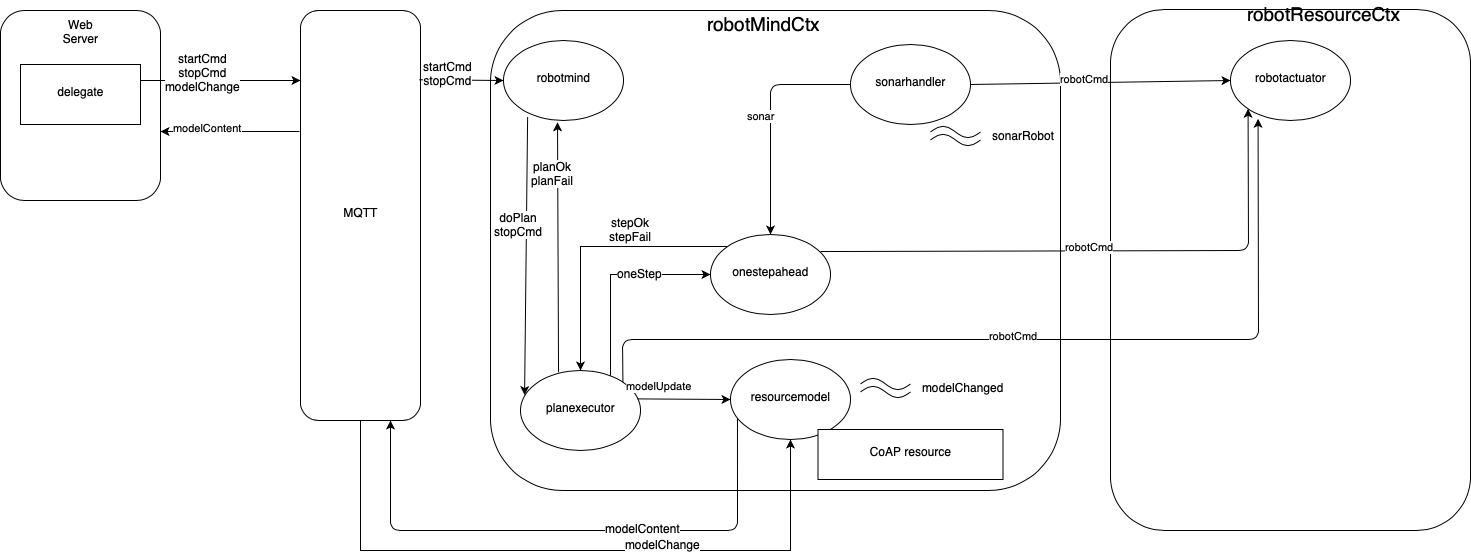
\includegraphics[width=\textwidth]{img/sprint4/arch_logica_4.png}
  \caption{L'architettura del sistema.}
  \label{fig:arch_logica_4}
\end{figure}


\subsection{Test plan}

Verificare il corretto funzionamento del sistema:

\begin{itemize}
\item durante la fase di esplorazione, quando il robot incontra un ostacolo, verificare che l'ostacolo venga segnalato correttamente sulla mappa;
\item una volta incontrato un ostacolo, verificare che il robot calcoli un nuovo piano per raggiungere il suo obiettivo;
\item verificare che, nel caso in cui l'obiettivo si trovi in corrispondenza di un ostacolo, il robot scelga il goal successivo senza bloccarsi;
\item verificare che, nel caso in cui un obbiettivo si trovi all'esterno dei confini il robot termini l'esplorazione;
\item verificare che, una volta determinati i confini della stanza, il robot esplori tutte le celle non ancora visitate;
\end{itemize}{}

\newpage
\section{Sprint 5} 

Il progetto di riferimento per questo sprint è it.unibo.ddrsystem6.

OBIETTIVO: creazione di un sistema con un robot che, una volta ricevuto il comando di start (R-starExplore), inizi a esplorare autonomamente la stanza in cui si trova (R-explore). Ogni volta che il robot incontra un ostacolo dovrà fermarsi(R-stopAtBag), scattargli una foto (R-takePhoto), inviarla alla console dell'operatore (R-sendPhoto) ed aspettare l'esito della verifica. In caso in cui la valigia risulti sospetta (ovvero contenete la bomba) il robot dovrà memorizzare la posizione della valigia (R-storePhoto), tornare alla propria base (R-backHomeSincePhoto).
In caso contrario dovrà continuare l'esplorazione (R-continueExploreAfterPhoto).

\subsection{Work Plan}
\begin{enumerate}
\item definizione di valigia sospetta;
\item definizione di "base del robot";
\item gestione dell'invio della foto di ogni ostacolo;
\item gestione della ricezione del messaggio contenente il risultato dell'analisi della bomba.
\end{enumerate}

\subsection{Analisi dei requisiti}

\textbf{Cosa si intende per valigia sospetta?}\\
Una valigia la si definisce sospetta quando, attraverso un tool esterno al sistema, si verifica se dentro di essa sia presente o meno una bomba. 

\textbf{Cosa si intende per "base del robot"?}\\
Il concetto di "base del robot" rimane invariato rispetto agli sprint precedenti: essa è il punto da cui il robot parte per esplorare la stanza. Nel caso specifico si è scelto l'angolo in alto a sinistra di una stanza, definito come (0,0).

\subsection{Analisi del problema}
\textbf{Come si deve comportare il robot quando incontra un ostacolo?}\\
Ogni volta che il robot incontra un ostacolo effettua un passo indietro per tornare nella cella precedente (backToCompensate). Tterminata questa fase, il robot si ferma ("R-stopAtBag"), scatta una foto ("R-takePhoto") ed infine la invia ("R-sendPhoto") al device dell'operatore. Infine il robot si mette in attesa di una risposta ("luggageSafe" or "luggageDanger"). 

\textbf{Cosa succede se la risposta ("luggageSafe" oppure "luggageDanger") non arriva mai al robot?}\\
Nel caso in cui il robot non riceva la risposta dalla console rimane fermo nella sua posizione.

\textbf{Cosa fa quando riceve il messaggio di "luggageDanger"?}\\
Quando riceve questo messaggio, significa che l'ultima valigia esaminata è quella contenete la bomba, dunque  il robot dovrà tornare alla base ("R-backHomeSinceBomb"). 

\textbf{Cosa fa quando riceve il messaggio di "luggageSafe"?}\\
Quando riceve questo messaggio, significa che l'ultima valigia esaminata non contiene la bomba, dunque  il robot dovrà continuare l'esplorazione e la verifica delle altre valigie ("R-continueExploreAfterPhoto"). 

\textbf{Come faccio a mostrare ed aggiornare le informazioni della valigia sulla web page?}
Per la visualizzazione dello stato della valigia corrente si è deciso di utilizzare le informazioni gestite dalle plannerUtils. La risorsa verrà rappresentata sulla web page nel seguente modo:
\texttt{luggage(photo\_id, position(X,Y), date\_time)}\\
Dove:
\begin{itemize}
    \item photo\_id rappresenta la foto della valigia scatta dal robot;
    \item position(X,Y) le coordinate della valigia nella mappa del robot;
    \item la data e l'ora in cui è stata scattata la foto;
\end{itemize}

Lo stato dell'ultima valigia mostrato sulla web page sarà quello relativo alla valigia con la bomba.

\subsection{Model}

Il committente richiede di salvare le informazioni della valigia sospetta (immagine, posizione, ora). Dato che inizialmente non si sa quale sia la bomba e la sua posizione, si ritiene importante salvare le informazioni solamente della valigia da ispezionare attualmente e:
\begin{itemize}
    \item nel caso in cui la verifica risulti negativa alla verifica da parte del tool le informazioni verranno sovrascritte da quelle della valigia seguente;
    \item altrimenti verranno salvate esattamente quelle della valigia sospetta.
\end{itemize}

Queste informazioni si potrebbero tener dentro al sistema (ad esempio per motivi di sicurezza o efficienza) oppure si potrebbero rendere accessibili da altri osservatori utilizzando la stessa strategia utilizzata per lo stato del robot e della stanza. Quest'ultima strategia potrebbe essere più efficace in quanto, essendo il tool utilizzato per la verifica esterno al sistema, potrebbe accedere a tali informazioni attraverso uno standard (CoAP) in maniera più trasparente che un messaggio "custom" della SoftwareFactory QKActor. 
Allo stesso tempo la risorsa potrebbe (la valigia) avere un attributo chiamato "safe" settato di default a "true" e a "false" dal tool di verifica. 
Dunque anche il nostro sistema dovrà essere un observer di tale risorsa in quanto, quando viene cambiato questo attributo, il sistema deve eseguire tutte le azioni descritte in precedenza. Tuttavia tale soluzione risulta superflua, dato che, è richiesto il salvataggio solo della valigia sospetta.
Il Listing \ref{lst:robotmind-ddr-sys-6} contiene la logica di gestione degli ostacoli della robtmind.

\begin{lstlisting}[backgroundcolor=\color{white}, label={lst:robotmind-ddr-sys-6}, caption={"Codice di robotmind in ddrSystem6"}]

QActor robotmind context robotMindCtx {

...

    State newLuggageFound {
    	//println("========== robotmind: newLuggageFound ==========")
    	["Luggage_num++"]
    	forward resourcemodel -m modelUpdate: modelUpdate(luggage, $Luggage_num)
    
    	run itunibo.planner.moveUtils.setObstacleOnCurrentDirection(myself)
    	["Map =  itunibo.planner.plannerUtil.getMapOneLine()"]
    	forward resourcemodel -m modelUpdate:modelUpdate(roomMap, $Map)
    	
    	
    	
    }
    Transition t2 whenMsg luggageSafe -> handleObstacle
    			  whenMsg luggageDanger -> endExploration
    
    
    State handleObstacle {
    	//println("========== robotmind: handleObstacle ==========")
    	run itunibo.planner.moveUtils.setObstacleOnCurrentDirection(myself)
    	run itunibo.planner.plannerUtil.resetGoal(X,Y)
    	run itunibo.planner.moveUtils.setObstacleOnCurrentDirection(myself)
    	["plan = itunibo.planner.plannerUtil.doPlan()"]
    }
    Goto startExploration if "(plan != null)" else checkNull
}
\end{lstlisting}


Ogni qualvolta la console viene notificata della presenza di un ostacolo, sulla web page si attivano due bottoni ("safe" e "dangerous") che permettono all'operatore di segnalare al sistema se l'ostacolo è pericoloso oppure no. Dopo che l'operatore ha premuto uno dei due bottoni, entrambi si disattivano fino all'ostacolo successivo.
Il Listing \ref{lst:appl-code-frontend} contiene la PUT fatte alla risorsa CoAP nel progetto frontend (classe applCode.js).
\begin{lstlisting}[backgroundcolor=\color{white}, label={lst:appl-code-frontend}, caption={"Put alla risorsa CoAP nel progetto frontend"}]


app.post("/danger", function(req, res,next) { handlePostMove("danger","going to initial position", req,res,next); });
app.post("/safe", function(req, res,next) { handlePostMove("safe","continuing the exploration", req,res,next); });

\end{lstlisting}

L'architettura del sistema rimane per lo più invariata rispetto allo sprint precedente. Gli unici messaggi che vi sono in più sono quelli utilizzati per segnalare la presenza di ostacolo pericoloso o meno (lato web page, tali messaggi corrispondono a delle PUT, con "safe" o "danger", alla risorsa CoAP).

\subsection{Test plan}

Verificare il corretto funzionamento del sistema:

\begin{itemize}
\item verificare che il robot, una volta incontrato un ostacolo, si metta in attesa del messaggio dell'operatore;
\item verificare che il robot, una volta ricevuto il messaggio di "luggageSafe", continui l'esplorazione della stanza;
\item verificare che il robot, una volta ricevuto il messaggio di "luggageDanger", torni alla base terminando la fase di esplorazione e senza verificare le celle non ancora visitate.
\end{itemize}{}





\newpage
\section{Sprint 6}

Il progetto di riferimento per questo sprint è it.unibo.ddrsystem6.

OBIETTIVO: creazione di un sistema con un robot che  una volta ricevuto il comando di "start", inizi a esplorare autonomamente la stanza in cui si trova solo se la temperatura della stanza è al di sotto di una certa soglia (R-tempOk). Una volta iniziata la fase di esplorazione, non appena la temperatura della stanza supera la soglia il robot si deve fermare. 
Durante l'esplorazione, se il robot riceve il comando di backHome (R-backHome), il robot deve sospendere l'esplorazione e tornare alla base.
Durante l'esplorazione il robot deve anche far blinkare un led (R-blinkLed).

Work plan:
\begin{enumerate}
\item definizione di una strategia con cui poter controllare la temperatura della stanza;
\item gestione del cambio di temperatura nel caso in cui essa superi una certa soglia;
\item gestione del messaggio di "backHome";
\item gestione del blinking del led posto sul robot durante la fase di esplorazione.
\end{enumerate}

\subsection{Analisi dei requisiti}

\textbf{Cosa si intende per variazione della temperatura della stanza?}
Per variazione della temperatura della stanza si intende un cambiamento significativo di essa che la porti ad assumere un valore superiore o inferiore ad una soglia fissata. 

\textbf{Cosa si intende per blinking del led?}\\
Per blinking del led si intende, nel caso del robot fisico, l'accensione ad intermittenza un led posto su di esso. Nel caso del robot simulato tale comportamento è simulato con una stampa su console ("blinking").

\subsection{Analisi del problema}

\textbf{Come è possibile gestire la variazione della temperatura della stanza?}\\

La variazione è gestita utilizzando due bottoni "OK" e "TOOHIGH". Quando il primo viene premuto significa che la temperatura è al di sotto di una certa soglia e non sono state rilevate variazioni particolarmente significative (temperatura accettabile). Invece, quando viene premuto il secondo bottone significa che vi è stata una variazione della temperatura tale da comportare l'arresto dell'esplorazione (temperatura alta).
Ad inizio esplorazione si ipotizza che la temperatura della stanza sia corretta. Una volta che  il bottone "TOOHIGH" viene premuto, il robot deve sospendersi in attesa che la temperatura ritorni nella norma (premendo il bottone "OK") e che l'operatore ridia il comando di "start".

\textbf{Come è possibile gestire il comando di "backHome"?}\\
L'esplorazione del robot è suddivisa nel raggiungimento di diversi goal. (i.e. (0,0)(1,1)(2,2)...) Quando l'operatore spinge il bottone di "backHome" è sufficiente indicare al robot che il goal da perseguire corrisponde alla propria base (0,0) e una volta che lo ha raggiunto aspettare che l'operatore ridia il comando di "start" per riprendere l'esplorazione. 

\textbf{Come è possibile gestire il blinking del led?}\\
Il task del blinking, pur essendo una funzionalità a parte rispetto a quella di esplorazione, deve comunque essere gestito in contemporanea rispetto a quest'ultimo. Quindi potrebbe risultare utile incapsulare tale comportamento in un'entità separata


\subsection{Model}

Per quanto riguarda la gestione della temperatura, è necessario modificare il behaviour del QKActor robotmind. Robotmind, sia prima di iniziare l'esplorazione, sia mentre questa è in corso, controlla se nel sistema si verifica un evento di "temperatureTooHigh". Nel primo caso, se ciò accade, il robot dovrà aspettare che si verifichi l'evento di "temperatureOk" e un comando di "start" prima di dare il via all'esplorazione. Nel secondo caso, il robot, arresta momentaneamente l'esplorazione sospendendo il piano che stava svolgendo, ponendosi prima in attesa dell'evento "temperatureOk" e poi del comando di "start" che gli consenta di riprenderla. Nel caso l'evento di "temperatureOk" non arrivi mai, il robot rimarrà fermo nella sua posizione attuale.
Il listing \ref{lst:robotmind_ddr_sys_6_temp} riporta il codice per gestire la logica applicativa della temperatura.


\begin{lstlisting}[backgroundcolor=\color{white}, label={lst:robotmind_ddr_sys_6_temp}, caption={Codice di QActor robotmind in ddrSystem6} ]
Event temperatureTooHigh: temperatureTooHigh

QActor robotmind context robotMindCtx {

	State waitForStart {
		...
	}

	Transition t0  whenEvent startCmd  -> startExploration
				   whenEvent temperatureTooHigh  -> waitForTemperatureOk
   
    ...
    
    State startExploration {
    	...
		
	} 

	Transition t1 whenEvent temperatureTooHigh -> waitForTemperatureOk
	              ...

    State backHome {
		   println("========== robotmind: backHome ==========")	  
		  forward planexecutor -m stopPlan: stopPlan
		  run itunibo.planner.plannerUtil.setGoal(0,0)
		  forward planexecutor -m doPlan : doPlan(0,0)   
	}
	Transition t2 whenEvent temperatureTooHigh  -> waitForTemperatureOk
	              ...
	              
	State handleStartAfterBackHome { }
	Transition t0  whenEvent temperatureTooHigh  -> waitForTemperatureOk
	                ...
	
	              
\end{lstlisting}

Quando l'operatore clicca il pulsante "backHome" sulla propria console tale evento viene catturato dal QKActor robotmind quando quest'ultimo si trova nello stato "startExploration". Una volta catturato tale evento prima di tutto interrompe il piano attualmente in esecuzione e poi imposta il nuovo goal a (0,0) in modo da tornare alla base. Una volta terminato il goal, robotmind, si mette in attesa dello "start". Nel caso in cui, durante tutto il procedimento, dovesse percepire l'evento di "stopCmd" oppure di "temperatureTooHigh", sospenderà l'esecuzione del compito per attendere gli opportuni comandi prima di ricominciare.
Il listing \ref{lst:backHome-ddr-sys-6} riporta il codice per gestire la logica applicativa del backHome.

\begin{lstlisting}[backgroundcolor=\color{white}, label={lst:backHome-ddr-sys-6}, caption={"Codice di robotmind per la gestione del backHome"}]

State startExploration {... } 

	Transition t1 ...
	             whenEvent backHomeCmd -> backHome

	State backHome {
		  forward planexecutor -m stopPlan: stopPlan
		  run itunibo.planner.plannerUtil.setGoal(0,0)
		  forward planexecutor -m doPlan : doPlan(0,0)   
	}
	Transition t2 whenMsg planOk -> handleStartAfterBackHome 
			      whenMsg planFail -> backHome
			      whenEvent stopCmd -> waitForStart
			      whenEvent temperatureTooHigh  -> waitForTemperatureOk
	
	State handleStartAfterBackHome {	}
	Transition t0  whenEvent startCmd  -> startExploration
				   whenEvent temperatureTooHigh  -> waitForTemperatureOk

\end{lstlisting}



Dal momento che si è individuato il compito del blinking del led come task separato rispetto a quello dell'esplorazione, ma che deve comunque essere svolto contemporaneamente, si è deciso di assegnare la gestione di tale compito ad un QKActor diverso da robotmind, denominato blinkinghandler. Tale attore, ogni volta che riceve il messaggio di "startBlinking" dovrà comunicare al robotactuator di iniziare il compito del blinking, e quando riceve il messaggio di stopBlinking, dovrà comunicare al robotactuator di terminarlo.
Dati i requisiti, la robotmind indicherà al blinkinghandler di avviare tale task non appena inizia la fase di esplorazione e di terminarlo quando viene individuata la valigia con la bomba.
Il listing \ref{lst:blinking-ddr-sys-6} riporta il codice per gestire la logica applicativa del blinkingLed.


\begin{lstlisting}[backgroundcolor=\color{white}, label={lst:blinking-ddr-sys-6}, caption={"Codice di blinkinghandler in ddrSystem6"}]

QActor blinkinghandler context robotMindCtx {
	
		State s0 initial {		}
		Transition t0 whenMsg startBlinking -> sendBlinkingMsg
		
		State sendBlinkingMsg{
			println("========== blinking ==========")
			forward robotactuator -m robotCmd : robotCmd (blinking)
		}
		Transition t1 whenMsg stopBlinking -> stopBlinking
		
		State stopBlinking{
			println("========== stop blinking ==========")
			forward robotactuator -m robotCmd : robotCmd (stopBlinking)
		}		
		Goto s0
}
\end{lstlisting}


In questo sistema si è revisionata anche la strategia di esplorazione: ora il robot, terminata una "chiocciola", prima di passare a quella successiva, esplora tutte le caselle a "0" presenti, senza esplorarle tutte una volta trovate le pareti. Questa nuova strategia permette di trovare un'eventuale bomba "as soon as possible".


L'architettura del sistema è riportata in \cref{fig:arch_logica_6}.

\begin{figure}[H]
  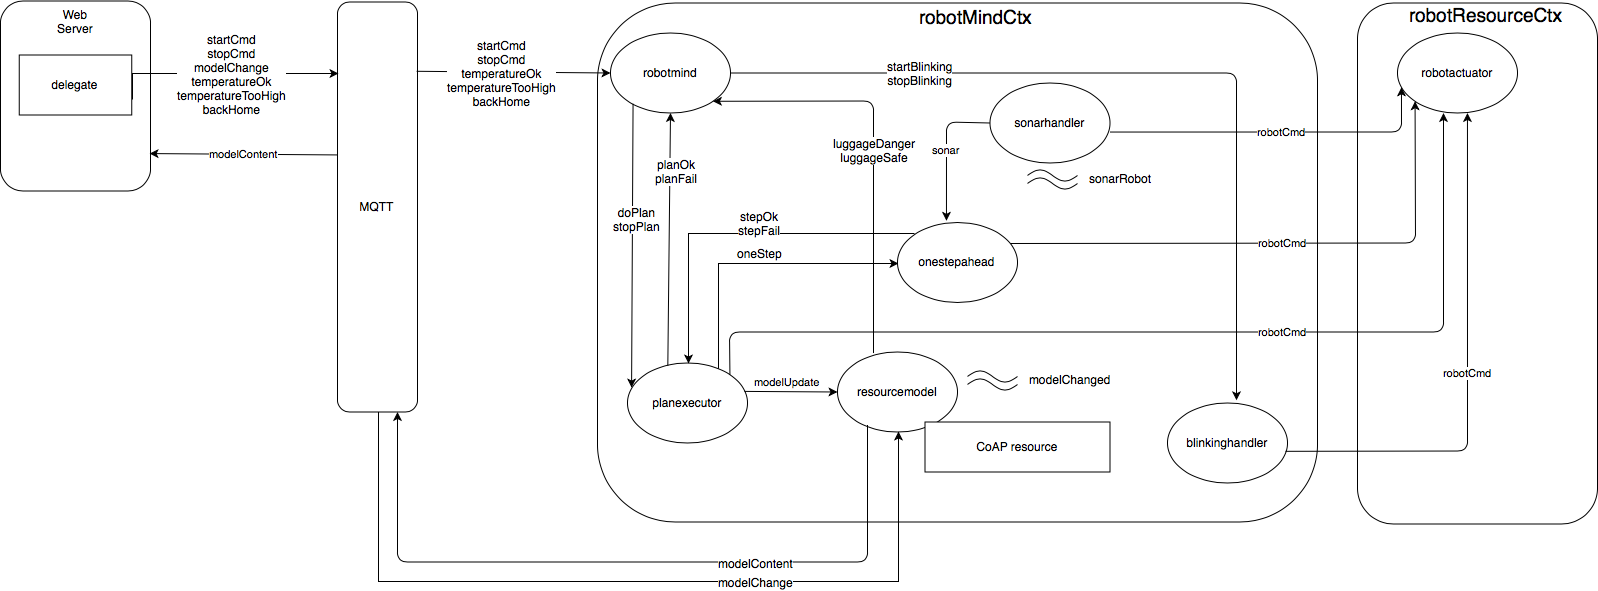
\includegraphics[width=1.7\textwidth, angle=270]{img/sprint6/arch_logica_6.png}
  \caption{L'architettura del sistema.}
  \label{fig:arch_logica_6}
\end{figure}



\subsection{Test plan}

Verificare il corretto funzionamento del sistema:

\begin{itemize}
\item verificare che il robot, una volta percepito l'evento di "temperatureTooHigh", sospenda l'esplorazione;
\item verificare che il robot, una volta sospesa l'esplorazione a seguito dell'evento "temperatureTooHigh" la riprenda solo una volta percepiti in ordine gli eventi "temperatureOk" e "startCmd":
\item verificare che il robot, una volta ripresa l'esplorazione dopo averla interrotta a causa della temperatura oltre la soglia, reimposti il goal corretto, ossia quello che stava svolgendo prima di fermarsi;
\item verificare che il robot, una volta percepito l'evento di "backHome", imposti il goal a (0,0);
\item verificare che il robot, una volta tornato alla base poiché ricevuto il comando di "backHome", si metta in attesa del comando di "start";
\item verificare che il robot, una volta ripresa la fase di esplorazione, dopo averla interrotta a causa del comando di "backHome", reimposti il goal corretto: quello che stava svolgendo prima di impostare (0,0);
\item verificare che il robot, non appena inizia la fase di esplorazione, avvi anche il blinking del led sul robot;
\item verificare che il robot, non appena termina la fase di esplorazione (o perché ha trovato la bomba o perché ha esplorato tutte le celle della stanza), termini anche il compito del blinking del led;
\end{itemize}{}


\newpage
\subsection*{Sprint0 Review }
\date{30/12/2018}\\
In questo sprint si sono definiti in modo formale i requisiti del sistema e si è analizzato in dettaglio il problema. 
Dall'analisi del problema è emersa l'architettura logica del sistema che è stata formalizzata utilizzando i QActor. %(file $code/LogicArchitecture.qa.tex$)

\subsection*{Sprint1 Review}
\date{27/06/2019}\\
In questo sprint si è modificato il sistema dello sprint0 in modo da permettere al robot di gestire (ricevere ed eseguire) i comandi base di spostamento: "vai avanti", "vai indietro", "gira a destra", "gira a sinistra", "fermati".  Ogni volta che esegue un comanda il sistema modifica coerentemente la sua base di conoscenza.

\subsection*{Sprint2 Review}
\date{15/07/2019}\\
In questo sprint si è modificato il sistema dello sprint1 in modo da permettere al robot (fisico e virtuale) di esplorare una stanza rettangolare e vuota. Durante l'esplorazione il robot costruisce internamente una rappresentazione della stanza (utilizzando le plannerUtils). Essendo la stanza vuota, l'unico ostacolo modellato in questo sistema sono i muri. Quando il robot riconosce un muro (attraverso l'uso di un sonar), esso fa un passo indietro, si ferma, salva l'informazione sulla mappa e procede con il goal seguente. 

\subsection*{Sprint3 Review }
\date{11/08/2019}\\
In questo sprint si è modificato il sistema dello sprint2 in modo da permettere al robot virtuale di partire con l'esplorazione automatizzata della stanza quando questa viene azionata sulla web page tramite il bottone start. Inoltre, si è creata una risorsa CoAP che rappresenti lo stato del robot e della stanza, il quale sarà osservabile direttamente sulla web page e aggiornato ogni qualvolta si modifichi.

\subsection*{Sprint4 Review }
\date{29/08/2019}\\
In questo sprint si è modificato il sistema dello sprint3 in modo da permettere al robot virtuale di esplorare autonomamente una stanza che contiene ostacoli fissi diversi dai muri (valigie). Questo ha richiesto di effettuare il refactoring dei diversi task assegnati precedentemente i QKActor. In particolare si è incapsulata in un nuovo attore (planexecutor) la gestione dell'attuazione di singolo un piano, e si è esteso il comportamento di robotmind modificando la logica applicativa del nuovo sistema. 

\subsection*{Sprint5 Review }
\date{4/09/2019}\\
In questo sprint si è modificato il sistema dello sprint4 in modo da permettere al robot virtuale di esplorare autonomamente una stanza che contiene ostacoli fissi diversi dai muri (valigie). In questo sistema, ogni volta che il robot incontra un ostacolo, si sospende in attesa dell'esito della verifica, con la relativa gestione di entrambe le casistiche.  Questo ha richiesto di modificare la logica applicativa incapsulata nel comportamento di robotmind: tale attore ora starà in attesa di ricevere due possibili messaggi: "luggageSafe" o "luggageDanger".

\subsection*{Sprint6 Review}
\date{12/09/2019}\\
In questo sprint si è modificato il sistema dello sprint5 in modo da permettere al robot virtuale di esplorare autonomamente una stanza che contiene ostacoli fissi. In questo sistema, ogni volta che la temperatura della stanza diventa più alta di una soglia, il robot si ferma in attesa che la temperatura si abbassi e che l'operatore gli ridia il comando di "start".
Durante l'esplorazione, quando l'operatore manda il comando di "backHome", il robot sospende il goal corrente per tornare alla base e attendere di nuovo il comando di "start", così da riprende l'esplorazione da dove l'aveva lasciata.
Durante tutta la fase di esplorazione il robot esegue anche un altro compito: far blinkare un led posto su di esso.
In questo sistema si è modificata la logica applicativa incapsulata nel comportamento di robotmind: tale attore ora potrà percepire anche gli eventi di: "temperatureTooHigh", "temperatureOk" e "backHome". 
Si è aggiunto un attore blinkinghandler per la gestione del blinking del led: quest'ultimo comincia la fase di blinking non appena riceve il messaggio di "startBlinking" e la termina quando riceve quello di "stopBlinking". "startBlinking" e "stopBlinking" sono entrambi messaggi inviati da robotmind.

%formato messaggi: msg( MSGID, MSGTYPE, SENDER, RECEIVER, CONTENT, SEQNUM ) 

\newpage

\begin{itemize}

\section{DOMANDE}

\item scelte progettuali a livello di architettura: perché e quali?

In base all'analisi dei requisiti e del problema, si è pensato di 
    - realizzare un sistema distribuito (console e robot, le diverse parti che girano su nodi diversi) e eterogeneo (sistemi qakactor, node). per permettere alle varie parti di comunicare si utilizzano un modello basato su messaggi e eventi ( qkactor: dipsatch e event -> attore kotlin: coda di messaggi)
    - usare un'architettura esagonale (modello tipico dell'IoT), modello delle risorse al centro. tutte le modifiche al sistema sono precedute da una modifica al modello delle risorse (es. model change inviati a resourcemodel, resource model li manda a robotmind). 

\item  Collegare le scelte progettuali ai principi studiati durante il corso (model driven development, "non c'é codice senza progetto", le fasi Scrum, la software factory ecc).

model driven development (a mano o automatizzato)-> è modalità di sviluppo software, cambio modello -> cambia codice \\
software factory -> tool con metalinguaggio che genera codice 
non c'è codice senza progetto, non c'è progetto senza analisi del problema, non c'è analisi del problema senza analisi dei requisiti -> abbiamo usato questo approccio nel codice e nella rel\\
fasi scrum -> scrum è metodologie Agile. È  definita da Ruoli (product owner, scrum master, team di sviluppo), Artefatti (Product Backlog - inizio -, Sprint Backlog - ogni sprint, e Incremento) ed Eventi (Sprint Planning, Daily Scrum, Sprint Review, Sprint Review, Retrospective).\\
 
\item Qual è la differenza tra analisi dei requisiti e analisi del problema? 
analisi dei requisiti -> COSA
analisi del problema -> COME, problematiche

(la differenza non è marcata da una linea netta ma suscettibile di varie interpretazioni e spiegare)

\item Qual è l’architettura logica del sistema? 
foglio stampato 

\item Da quante parti è composto il vostro sistema?

2 contesti (nodi) + 1 console in remoto 

\item Spiegare perché avete evocato un certo concetto in una fase piuttosto che nell'altra?
(l'importante in questo caso è avere le idee chiare e saper fornire un ragionamento logico)

\item Qual è il rapporto (quindi interazione) tra i componenti del sistema?

messaggi e eventi: fra web server e  contesto della mind (eventi sparati sulla topic qak/events, messaggi inviati sulla topic del qkactor)
messaggi: da contesto della mind a contesto actuator
	
\item Che modello delle risorse avete usato? Come funziona?
informazioni sullo stato robot 

Nel nostro progetto il modello delle risorse è gestito mediante le plannerUtils. In particolare:

Rombo pieno = composizione (persona, cuore -> la persona non eistenza senza cuore)
rombo vuoto = aggregazione (casa, divano -> la casa esiste anche senza divano)

Per rendere le risorse accessibili via web abbiamo utilizzato CoAP (il resourcemodel manda updatemodel(che emette evento modelContent (MQTT) e aggiorno risorsa CoAP)).

\begin{figure} [H]
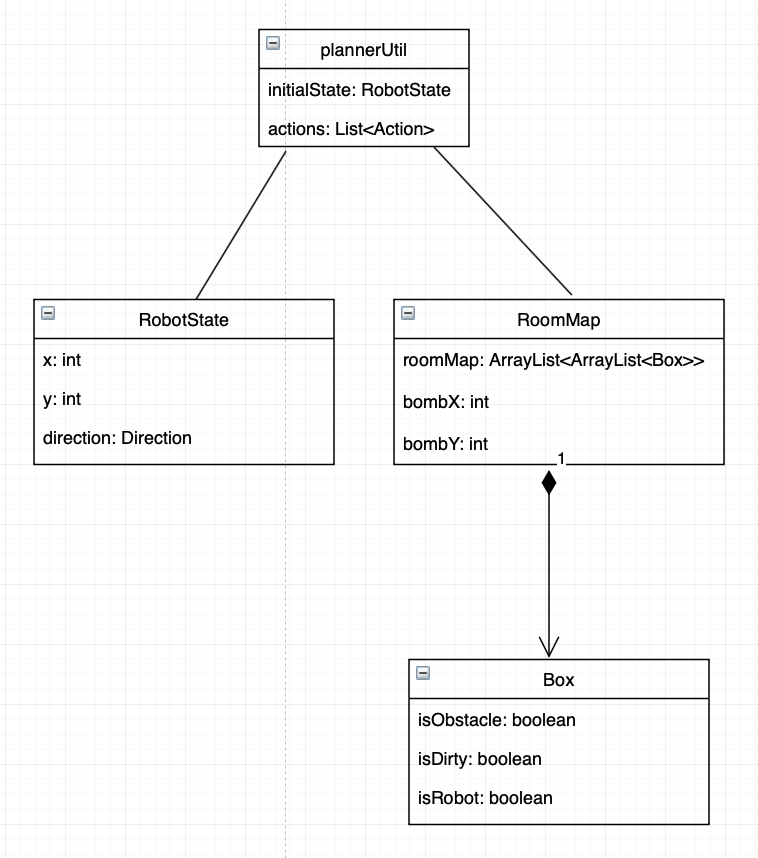
\includegraphics[width=\linewidth]{img/modello_risorse_java.png}
\end{figure}


\item Come avete fatto la rappresentazione della base di  conoscenza?

- inizio, prolog -> rappresentavamo solo stato del robot \\
- poi, tolto prolog -> abbiamo usato le plannerUtils -> rappresentavamo stato del robot, mappa e bagaglio
(non dire: la temperatura non la salviamo nelle plannerUtils)

\item Problema della consistenza: come mantenete la consistenza tra modelli delle risorse diversi?


Unico modello delle risorse (gestito in PlannerUtils).\\

consistenza tra PlannerUtils e CoAP.\\

ogni volta che cambiamo qualcosa nelle PlannerUtils, l'attore resourceModel aggiorna la risorsa CoAP (non dire: di fatto lo fa mandando un modelContent a MQTT)\\

\item Come è gestita l’interazione tra i diversi attori? 

riguardare i messaggi che si scambiano tra attori 

\item Il framework dei qactor è message based/driven, event based/driven?

message based, event based/driven

\item test plan: cosa sono e quando vanno fatti?
servono a verificare la correttezza del sistema in maniera automatzzata.
(posso sia implementarli prima di fare l'imple o anche dopo, se prima -> non funzioneranno)

\item Struttura, comportamento e interazione per ogni componente del sistema?

\item Struttura, comportamento e interazione per il sistema?
Struttura del sistema su quale nodo (contesto) mi trovo,
comportamento degli attori, 
interazione -> comunicazione con messaggi e eventi nel sistema

\item Come usate MQTT? Perché avete usato MQTT? E non, ad esempio, TCP?
MQTT per gestire scambio di messaggi (eventi gestiti sulla topic come messaggi), usa patter publish/subscribe e fornisce delle astrazioni più ad alto livello. 

\item Come usate CoAP? Perché avete usato CoAP?

rendere disp. via web. le info del nostro sistema. CoAP è : implementazione del protocollo restfull + usato in ambito iot.

\item Quali sono le parti del vostro sistema fisico?

-l'applicazione web\\
-l'applicazione che gestisce la logica del sistema\\
-l'applicazione che gestisce robot fisico/virtuale\\


\item  Tutta la storia sul progetto: architetture di progetto, goal e vision (bottom up, top down)

\item Perché strategia a chiocciola e non altre? es. a colonne, a righe,...
perché permette di esplorare in maniera omogenea incrementale la stanza 

\item nostro progetto approccio top down -> prima interazione poi comportaemtno. bottom up sarebbe stato contrario

\item per fare arch. logica devo decidere: quanti compoennti ha il sistema e la loro interazione (definisco formato messaggi)
\end{itemize}
\end{document}
